\chapter{Learning data from a resolved liquid jet in crossflow}
	\label{ch5:jicf_resolved_simulations}



Describe here all our simulations done with JICF, what we have achieved with them, etc.

\begin{itemize}

	\item Experimental setup description
	
	\item Numerical setup description. Operating points
	
	\item Mesh convergence study
	
	\item Spray sampling
	
	\item Direct measurement of fluxes with interior boundaries
	
	\item Liquid disappearing (set levelset band ) ??
	
	\item Results:
	
		\begin{itemize}
		
			\item Breakup mechanisms
			
			\item In-nozzle phenomena of flow separation (and entrainment of gaseous bubbles)
			
			\item Spray formation and evolution with axial distance
	
		\end{itemize}
		
	\item Other results:
	
		\begin{itemize}
		
			\item Slip velocity evolution
			
			\item Vorticity distribution (horse-shoe vortices, double vortical structural in liquid)
		
		\end{itemize}

\end{itemize}

\newpage 

\section{Introduction}

The previous chapter has detailed the theory of the proposed models to build lagrangian injectors for initialising dispersed phase simulations, named Smart Lagrangian Injectors (SLI). These models, nowadays in its earliest state of maturity, are intended to be generic and applicable to a broad range of operating conditions and injector configurations. To show its capabilities, they have been developed in their first stage with resolved simulations of liquid jet in crossflow (JICF) configuration. This chapter details these simulations, performed with the software YALES2 (\textbf{ref:2011-moureau-design}). % \textbf{https://reader.elsevier.com/reader/sd/pii/S1631072110002111?token=9137B6903478D4E8E427F5D8218DFC3EB42446DB034970B14BA9DE87AA7E80D130124A7EF8D8608D21D5D465CCE05A4F&originRegion=eu-west-1&originCreation=20210524114835}

The fundamentals and the physics of non-reactive JICF have been introduced in $\S$\ref{sec:ch1_fuel_injection_technology}. This chapter shows the results, analysis and injectors obtained from a kerosene JICF simulation replicating the experimental facility tested by \citeColor[becker_breakup_2002]. This configuration is used for validating the models. Section \ref{sec:ch5_experimental_bench} displays the experimental test bench, whose numerical setup and operating conditions chosen for numerical computations are detailed in Section \ref{sec:computational_setup}.


\section{Experimental test case}
	\label{sec:ch5_experimental_bench}

The experimental configuration tested by \citeColor[becker_breakup_2002] is shown in Figure \ref{fig:experiment_JICF_DLR}. The test rig is shown at the left. Liquid kerosene is injected through the atomizer ports to a quartz glass duct of rectangular cross section $25$x$40$ mm$^2$. The duct inlet is located at $120$ mm upstream the injection port. The boundary layer thickness developing along the bottom of the duct has been measured experimentally just upstream the atomizer, being between $4$ and $5$ mm. The lateral walls allow for optical access from the atomizer port until a location at 100 mm downstream. Air is introduced through two separate channels, a main one and a supplementary one. The main airflow is injected at the inlet of the quartz duct, while the supplementary one passes around it. Both airflows merge at the end of the duct and leave the domain through a common exit acting as a sonic throttle. The velocity inside the quartz can then be tuned by varying the size of the nozzle and the supplementary air flow rate. In the experiments performed, the range of air velocities goes from $u_g = 50$ to 100 m/s and the range of pressure from $p$ = 1.5 to 15 bar, hence allowing the study high-pressure conditions. The air temperature is maintained to $T_g = 290$ K. The fuel tested was kerosen Jet A-1 with density $\rho_l = 795$ kg m$^{-3}$ and surface tension $\sigma = 22 \cdot 10^{-3}$ N m$^{-1}$.

The liquid injection nozzle can be seen in Figure \ref{fig:experiment_JICF_DLR} right. It consists of a plain jet nozzle of $d_\mathrm{inj} =  0.45$ mm diameter and $L/d_\mathrm{inj}$ ratio of 1.56 with sharp edges. The average discharge coefficient for the mass flow rates of interest in the experimental studies is $0.6$. More details on the test rig can be found in \citeColor[brandt_experimental_1997].

\begin{figure}[h!]
	\centering
	\includegraphics[scale=0.45]{./part2_developments/figures_ch5_resolved_JICF/experiment_JICF_DLR}
	\caption[JICF experimental setup]{JICF experimental setup. \textsl{Left}: Test rig. \textsl{Right}: liquid nozzle geometry employed in the experimental study. Source: \citeColor[becker_breakup_2002]}
	\label{fig:experiment_JICF_DLR}
\end{figure}


A correlation for the trajectory of the jet was obtained experimentally by analysing optically its penetration for the several operating conditions tested. It corresponds to the trajectory of the jet's windward side, and gives a relation between the vertical location $z$ with respect to the axial coordinate $z$ as a function of the nozzle diameter $d_\mathrm{inj}$ and the momentum ratio $q$ defined by Eq. (\ref{eq:q_and_We_JICF_parameters}): % The rorrelation has a standard deviation of 0.81.

\begin{equation}
    \label{eq:jicf_trajectory_becker}
    \frac{z}{d_\mathrm{inj}} = 1.57 \mathrm{q}^{0.36} \ln \left( 1 + 3.81 \frac{x}{d_\mathrm{inj}} \right)
\end{equation}



\section{Computational setup}
	\label{sec:computational_setup}

\subsection*{Numerical domain}

Figure \ref{fig:numerical_setup_maquette_JICF_DLR} shows the computational domain developed to replicate the simulations of the test bench shown in Figure \ref{fig:experiment_JICF_DLR}. The duct is modelled as a plenum consisting of a box of dimensions 25x40x270 mm$^3$. The hydraulic diameter of the duct cross section, which is used to calculate the gas Reynolds number, is $D_h = 30.8$ mm. A magnified view of the nozzle is also shown, with diameter $0.45$ mm and straight section length of 0.7 mm prior to injection to keep $L/D = 1.56$ as in the experiments. The boundary conditions are also indicated. The plenum walls use a wall law of logarithmic type except closer to the domain pressure outlet, which have been set to slip walls to avoid backflow. The nozzle walls are rigid walls. For the liquid inlet, a Poiseuille profile has been specified, while in the gaseous inlet a velocity profile has been set in order to recover the boundary layer thickness of between 4 and 5 mm upstream the injection nozzle as described in the experiments (see Appendix \ref{app:JICF_BL_setup} for details). 

\begin{figure}[ht]
     \centering
     \includeinkscape[scale=0.4]{./part2_developments/figures_ch5_resolved_JICF/DLR_becker_numerical_config}
      \caption{Numerical domain and boundary conditions of the experimental test bench of \citeColor[becker_breakup_2002]. \textsl{Left}: complete domain. \textsl{Right}: detailed view of the injection nozzle. All dimensions are in mm.}
      \label{fig:numerical_setup_maquette_JICF_DLR}
\end{figure}

An overview of the baseline mesh is shown in Figure \ref{fig:jicf_dlr_mesh}. It is composed of 28 million tetrahedral cells. The baseline cell size in the channel is ??, while smaller elements have been located in the liquid nozzle. The region close to the injector has been refined. This mesh is used initially in all the simulations performed, and it will change dynamically as liquid is introduced in the domain due to the AMR routine. 

\begin{figure}[h!]
	\centering
	\includegraphics[scale=0.7]{./part2_developments/figures_ch5_resolved_JICF/jicf_dlr_mesh}
	\caption{Baseline mesh used for the JICF study. \colorbox{red}{OJO: de Felix. Sacar foto aqui!}}
	\label{fig:jicf_dlr_mesh}
\end{figure}

\subsection*{Operating conditions}

Two operating conditions tested experimentally in \citeColor[becker_breakup_2002] have been simulated. Both of them have the same momentum ration $q = 6$ but differ in the Weber number: $We_g = 830$ (low Weber) and $We_g = 1470$ (low Weber). According to the values of $q$ and $We_g$, the former condition corresponds to surface breakup dominating regime while the latter is located at the dividing line between column and surface breakup. Figure \ref{fig:location_JICF_ops_in_breakup_map} shows the location of both operating points in the breakup map of \citeColor[wu_breakup_1997]. The physical magnitudes and dimensionless numbers of both operating points are shown in Table \ref{tab:jicf_operating_conditions}. Apart from the values $q$ and $We_g$, the dimensionless numbers in  Eq. (\ref{eq:dimensionless_numbers_jicf}) are also calculated: the liquid and gaseous Reynolds numbers $Re_g$ and $Re_g$ respectively, Ohnesorge number $Oh$, aerodynamic Weber $We_\mathrm{aero}$, relative Weber $We_\mathrm{rel}$ and density ratio $r$. These numbers have been added since they are defined in several experimental studies \citeColor[wu_breakup_1997,becker_breakup_2002,ragucci_trajectory_2007] to characterize the operating points tested. 

For performing the computations of resolved atomization, the ACLS methodology combined with the AMR routine described in $\S$\ref{subsec:ch2_ACLS} is used. For each simulation, two interface mesh sizes have been simulated: $\Delta x_\mathrm{min} = 20 \mu m$ (coarse case) and $\Delta x_\mathrm{min} = 10 \mu m$ (fine case). Therefore, a total of four simulations have been done. The nomenclature for each simulation, which is used hereafter in this document, is introduced in Table \ref{tab:jicf_resolved_simulations_performed}.

%\begin{subequations}
%\label{eq:dimensionless_numbers_jicf}
%\begin{align}
%Re_l &= \frac{\rho_l u_l d_\mathrm{inj}}{\mu_l}\\
%Re_g &= \frac{\rho_g u_g D_h}{\mu_g}\\
%We_\mathrm{aero} &= \frac{\rho_g u_l^2 d_\mathrm{inj}}{\sigma}  \\
%We_\mathrm{rel} &= \frac{\rho_g \left( u_g - u_l \right)^2 d_\mathrm{inj}}{\sigma} \\
%Oh &=  \frac{\mu_l}{\sqrt{\rho_l \sigma d_\mathrm{inj}}}\\
%r &= \frac{\rho_l}{\rho_g} 
%\end{align}
%\end{subequations}

%\begin{align}
%\label{eq:dimensionless_numbers_jicf}
%Re_l &= \frac{\rho_l u_l d_\mathrm{inj}}{\mu_l}          &  Re_g &= \frac{\rho_g u_g D_h}{\mu_g}              &  Oh &=  \frac{\mu_l}{\sqrt{\rho_l \sigma d_\mathrm{inj}}}\\
%We_\mathrm{aero} &= \frac{\rho_g u_l^2 d_\mathrm{inj}}{\sigma}    &  We_\mathrm{rel} &= \frac{\rho_g \left( u_g - u_l \right)^2 d_\mathrm{inj}}{\sigma}          & r &= \frac{\rho_l}{\rho_g} 
%\end{align}


\begin{equation}
\label{eq:dimensionless_numbers_jicf}
\begin{aligned}
Re_l &= \frac{\rho_l u_l d_\mathrm{inj}}{\mu_l}          &  Re_g &= \frac{\rho_g u_g D_h}{\mu_g}              &  Oh &=  \frac{\mu_l}{\sqrt{\rho_l \sigma d_\mathrm{inj}}}\\
We_\mathrm{aero} &= \frac{\rho_g u_l^2 d_\mathrm{inj}}{\sigma}    &  We_\mathrm{rel} &= \frac{\rho_g \left( u_g - u_l \right)^2 d_\mathrm{inj}}{\sigma}          & r &= \frac{\rho_l}{\rho_g} 
\end{aligned}
\end{equation}

\begin{table}[!h]
\centering
\caption{JICF operating points studied}
\begin{tabular}{lcccc}
\thickhline
\textbf{Parameter} & \textbf{Symbol} & \textbf{Units} &  \textbf{Low Weber} &  \textbf{High Weber} \\ %\textbf{WE\_880} &  \textbf{WE\_1470} \\
\thickhline
Nozzle diameter & $d_\mathrm{inj}$ & mm & 0.45 & 0.45 \\
%\hline
Gas bulk velocity & $u_g$ & m s$^{-1}$ & 75 & 100 \\
%\hline
Liquid bulk velocity & $u_l$ & m s$^{-1}$ & 17.5  & 23.33 \\
%\hline
Liquid flow rate & $Q_l$ & mm$^3$ s$^{-1}$ & 2783  & 3710 \\
%\hline
Gas density & $\rho_g$ & kg m$^{-3}$ &  7.21 & 7.21 \\
%\hline
Liquid density & $\rho_l$ & kg m$^{-3}$ &  795 & 795  \\
%\hline
Gas viscosity & $\mu_g$ & kg m$^{-1}$ s$^{-1}$ & $1.8162 \cdot 10^{-5}$ &  $1.8162 \cdot 10^{-5}$  \\
%\hline
Liquid viscosity & $\mu_l$ & kg m$^{-1}$ s$^{-1}$ & $1.5 \cdot 10^{-3}$ & $1.5 \cdot 10^{-3}$  \\
%\hline
Surface tension & $\sigma$ & kg s$^{-2}$ &  0.022 & 0.022  \\
\thickhline
Momentum ratio & $q$ & - & 6 & 6 \\
%\hline
Gas Reynolds number & $Re_g$ & - & $0.92 \cdot 10^6$ & $1.22 \cdot 10^6$ \\
%\hline
Liquid Reynolds number & $Re_l$ & - & 4170 & 5560 \\
%\hline
Gas Weber number & $We_g$ & - & 830 & 1470 \\
%\hline
Liquid Weber number & $We_l$ & - & 5000 & 8850 \\
%\hline
Relative Weber number & $We_\mathrm{rel}$ & - & 490 & 870 \\
%\hline
Aerodynamic Weber number & $We_\mathrm{aero}$ & - & 45 & 80 \\
%\hline
Ohnesorge number & $Oh $ & - & 0.017 & 0.017 \\
%\hline
Density ratio & $r$ & - & 110 & 110 \\
%\hline
%Viscosity ratio & $\mu_l/\mu_g$ & [-] &  \multicolumn{2}{|c|}{1} \\
\thickhline
\end{tabular}
\label{tab:jicf_operating_conditions}
\end{table}

\begin{table}[!h]
\centering
\caption{Nomenclature for resolved atomization simulations}
\begin{tabular}{ccc}
\thickhline
%$\pmb{\Delta} x_\mathrm{min}$ [$\pmb{\mu}$$\textbf{m}])  &  \multicolumn{2}{c}{\textbf{Operating condition}} \\ 
$\Delta x_\mathrm{min}$ [$\mu$m]  &  \multicolumn{2}{c}{\textbf{Operating condition}} \\ 
\cline{2-3}
 &  Low $We_g$ &  High $We_g$ \\ 
\thickhline
\textbf{10} & UG75\_DX10 & UG100\_DX10 \\
\textbf{20} & UG75\_DX20 & UG100\_DX20 \\
\thickhline
\end{tabular}
\label{tab:jicf_resolved_simulations_performed}
\end{table}

\begin{figure}[ht]
     \centering
     \includeinkscape[inkscapelatex=false,scale=0.6]{./part2_developments/figures_ch5_resolved_JICF/jicf_breakup_regime_our_operating_points}
     \caption{Location of simulated operating conditions in the breakup map by \citeColor[wu_breakup_1997]}
	% See: https://stackoverflow.com/questions/35210337/can-i-plot-several-histograms-in-3d/35225919
      \label{fig:location_JICF_ops_in_breakup_map}
\end{figure}



%\section{YALES2 code (??)}

\section{Tools and methodologies}

%\subsection{Spray sampling in resolved simulations}

\subsection{Numerical computation of jet trajectory}
	\label{sec:ch5_jicf_trajectories}

As explained in $\S$\ref{sec:ch1_fuel_injection_technology}, one of the most important features of a jet in crossflow is its penetration. Experimental studies often provide correlations for the trajectory of the windward side of the jet (see Table \ref{tab:correlations_experimental_JICF}), such as the one from Eq. (\ref{eq:jicf_trajectory_becker}). These correlations depend on factors such as the momentum flux ratio $q$, the injection diameter $d_\mathrm{inj}$ and, in some case \citepColor[ragucci_trajectory_2007], in the Weber number $We$. The overall dependency of the trajectory on these parameters is still unknown and an ongoing research topic.

It is therefore of interest, to obtain the trajectory for the jet penetration in the performed resolved simulations. Several methods can be used for this purpose. This section describes four possible methodologies, two based on processing instantaneous trajectories and two based on processing the mean $\psi$ field. The results obtained with these methodologies are shown in $\S$\ref{sec:results_JICF_resolved}.

\subsubsection{Methods based on instantaneous trajectories}

One possible way of obtaining tra

\begin{figure}[ht]
     \centering
     \begin{subfigure}[b]{0.45\textwidth}
         \centering
         \includeinkscape[inkscapelatex=false,scale=0.35]{./part2_developments/figures_ch5_resolved_JICF/trajectories_obtention/instantaneous_interface_3D}
         %\caption{Instantaneous jet interface}
     \end{subfigure}
     %\hfill
     \begin{subfigure}[b]{0.45\textwidth}
         \centering
         \includeinkscape[inkscapelatex=false,scale=0.35]{./part2_developments/figures_ch5_resolved_JICF/trajectories_obtention/instantaneous_interface_y0}
         %\caption{Contour of instantaneous interface at plane y = 0}
     \end{subfigure}
        \caption{\textsl{Left}: instantaneous jet interface. \textsl{Right}: contour of instantaneous interface at plane y = 0}
	% See: https://stackoverflow.com/questions/35210337/can-i-plot-several-histograms-in-3d/35225919
        \label{fig:trajectory_obtention_instantaneous_general}
\end{figure}


%\subsubsection*{Non-monotonic trajectory}

\paragraph{{Non-monotonic trajectory}} 

This works well

\begin{figure}[ht]
     \centering
     \begin{subfigure}[b]{0.45\textwidth}
         \centering
         \includeinkscape[inkscapelatex=false,scale=0.35]{./part2_developments/figures_ch5_resolved_JICF/trajectories_obtention/method_a_sweep_nonMonotonic}
         %\caption{Instantaneous jet interface}
     \end{subfigure}
     %\hfill
     \begin{subfigure}[b]{0.45\textwidth}
         \centering
         \includeinkscape[inkscapelatex=false,scale=0.35]{./part2_developments/figures_ch5_resolved_JICF/trajectories_obtention/method_a_inst_trajectory}
         %\caption{Contour of instantaneous interface at plane y = 0}
     \end{subfigure}
        \caption{Obtention of non-monotonic instantaneous trajectory. \textsl{Left}: sweep process along z axis of interface points. \textsl{Right}: instantaneous trajectory.}
	% See: https://stackoverflow.com/questions/35210337/can-i-plot-several-histograms-in-3d/35225919
        \label{fig:trajectory_obtention_instantaneous_method_a}
\end{figure}


%\subsubsection*{Monotonic trajectory}
\paragraph{Monotonic trajectory} 

This works well too !


\begin{figure}[ht]
     \centering
     \begin{subfigure}[b]{0.45\textwidth}
         \centering
         \includeinkscape[inkscapelatex=false,scale=0.35]{./part2_developments/figures_ch5_resolved_JICF/trajectories_obtention/method_b_sweep_monotonic}
         %\caption{Instantaneous jet interface}
     \end{subfigure}
     %\hfill
     \begin{subfigure}[b]{0.45\textwidth}
         \centering
         \includeinkscape[inkscapelatex=false,scale=0.35]{./part2_developments/figures_ch5_resolved_JICF/trajectories_obtention/method_b_inst_trajectory}
         %\caption{Contour of instantaneous interface at plane y = 0}
     \end{subfigure}
        \caption{Obtention of monotonic instantaneous trajectory. \textsl{Left}: sweep process along z axis of interface points, excluding points whose vertical location is lower than the vertical location of the previous ones. \textsl{Right}: instantaneous trajectory.}
	% See: https://stackoverflow.com/questions/35210337/can-i-plot-several-histograms-in-3d/35225919
        \label{fig:trajectory_obtention_instantaneous_method_b}
\end{figure}


\subsubsection{Methods based on the mean levelset field}

Another possibility to obtain mean trajectories is by using the mean field of the levelset magnitude, $\overline{\phi}$. 

\paragraph{Maximum gradient method}

This method is more similar to the experimental methods presented in \citeColor[becker_breakup_2002] and \citeColor[freitag_spray_2008], since they obtain the trajectory as the contour giving the maximum intensity gradient in the vertical direction in processed images of the mean jet.

\begin{equation}
\max \left( \nabla \overline{\phi} \right)
\end{equation}

\paragraph{Trajectory as iso-contour of mean levelset}



\subsection{Direct measurement of liquid fluxes}
\label{subsec:ch5_interior_boundaries}



Droplet sampling is performed by tracking the center of mass of resolved structures and checking when it crosses the sampling planes. 


The sampling procedure of droplets is based on a lagrangian tracking of their center of mass. The position of the center of mass before and

In the ACLS simulations, a 

Liquid flow rates are calculated from the levelset function $\phi$ with the following equation:

\begin{equation}
Q_l = \int_{\partial \Omega} \phi \left( \textbf{u} \cdot \textbf{n} \right) dS
\end{equation}

where $\partial \Omega$ is the surface where integration is performed (i.e. the interior boundary), $\textbf{u}$ is the velocity and $\textbf{n}$ is the normal to the plane.


\begin{figure}[ht]
     \centering
     \includeinkscape[inkscapelatex=false,scale=0.6]{./part2_developments/figures_ch5_resolved_JICF/sampling_planes_with_IBs}
     \caption{Planes where fluxes are measured with interior boundaries. \colorbox{red}{Poner una imagen mas bonita} }
	% See: https://stackoverflow.com/questions/35210337/can-i-plot-several-histograms-in-3d/35225919
      \label{fig:jicf_interior_boundaries_surface_measurements}
\end{figure}


%\begin{figure}[ht]
%     \centering
%     \begin{subfigure}[b]{0.45\textwidth}
%         \centering
%         \includeinkscape[inkscapelatex=false,scale=0.35]{./part2_developments/figures_ch5_resolved_JICF/trajectories_obtention/instantaneous_interface_3D}
%         %\caption{Instantaneous jet interface}
%     \end{subfigure}
%     %\hfill
%     \begin{subfigure}[b]{0.45\textwidth}
%         \centering
%         \includeinkscape[inkscapelatex=false,scale=0.35]{./part2_developments/figures_ch5_resolved_JICF/trajectories_obtention/instantaneous_interface_y0}
%         %\caption{Contour of instantaneous interface at plane y = 0}
%     \end{subfigure}
%        \caption[Planes where fluxes are measured with interior boundaries.]{Planes where fluxes are measured with interior boundaries. \textsl{Left}: planes perpendicular to crossflow direction. \textsl{Right}: filming planes.}
%	% See: https://stackoverflow.com/questions/35210337/can-i-plot-several-histograms-in-3d/35225919
%        \label{fig:jicf_interior_boundaries_surface_measurements}
%\end{figure}
%


\section{Results}
\label{sec:results_JICF_resolved}



\subsection{Jet topology and breakup}

\subsubsection{Effect of mesh}

\subsubsection{Effect of operating point}

\subsection{Jet penetration: validation with experiments}


The accuracy of the mean numerical trajectories can be quantitatively assessed by defining a $L_2$ error as in Eq.~(\ref{eq:L2_JICF}): 

\begin{equation}
\label{eq:L2_JICF}
    L_2 = \sqrt{\frac{1}{N}   \sum_{i=1}^N \left( \frac{z}{d_\mathrm{inj}} \Bigr|_{\mathrm{exp},i} -   \frac{z}{d_\mathrm{inj}} \Bigr|_{\mathrm{num},i} \right)^2}
\end{equation}



\subsection{Characteristic times}

$\tau_\mathrm{lig}$ is the ligament stripping time from the liquid column.
$\tau_\mathrm{ph}$ is defined as:

\begin{equation}
\tau_\mathrm{ph} = \frac{d_\mathrm{inj}}{u_l}
\end{equation}



\begin{table}[!h]
\centering
\caption{Characteristic physical times in JICF simulations}
\begin{tabular}{ccc}
\thickhline
\textbf{Case} & $\tau_\mathrm{lig}$ & $\tau_\mathrm{ph}$ \\
\thickhline 
UG75\_DX10  & & \\
UG75\_DX20  & & \\
UG100\_DX10 & & \\
UG100\_DX20 & & \\
\thickhline
\end{tabular}
\label{tab:jicf_characteristic times}
\end{table}

We can also define characteristic times as droplets reach the sampling planes. For it, we can make a specific table for each case and each plane:

\begin{table}[!h]
\centering
\caption{Characteristic droplet times in JICF simulations}
\begin{tabular}{ccccc}
\thickhline
\textbf{Case} & $x = 5 mm$ & $x = 10 mm$ & $x = 15 mm$  & $x = 20 mm$ \\
\thickhline 
UG75\_DX10  & & & - & - \\
UG75\_DX20  & & & & \\
UG100\_DX10 & & & - & -\\
UG100\_DX20 & & & & \\
\thickhline
\end{tabular}
\label{tab:jicf_characteristic_droplet_sampling_times}
\end{table}



\subsection{Direct measurement of liquid flow rates}

Liquid fluxes have been measured in the resolved simulations at the planes shown in Figure \ref{fig:jicf_interior_boundaries_surface_measurements}. In the coarse simulations done with a mesh resolution of $\Delta x_\mathrm{min} = 20 \mu m$, fluxes have been obtained in all planes shown in the sketch. For the fine simulations, results were collected up to x = 10 mm since the liquid was removed shortly afterwards.

\subsubsection*{Obtention of total flow rate}

The time evolution of flow rates for case UG100\_DX20 is shown in Figure \ref{fig:IB_liquid_flow_rate_inst_evolution_UG100_DX20} for both crossflow and filming planes. For the crossflow planes, the 

%\begin{figure}[h!]
%\centering
%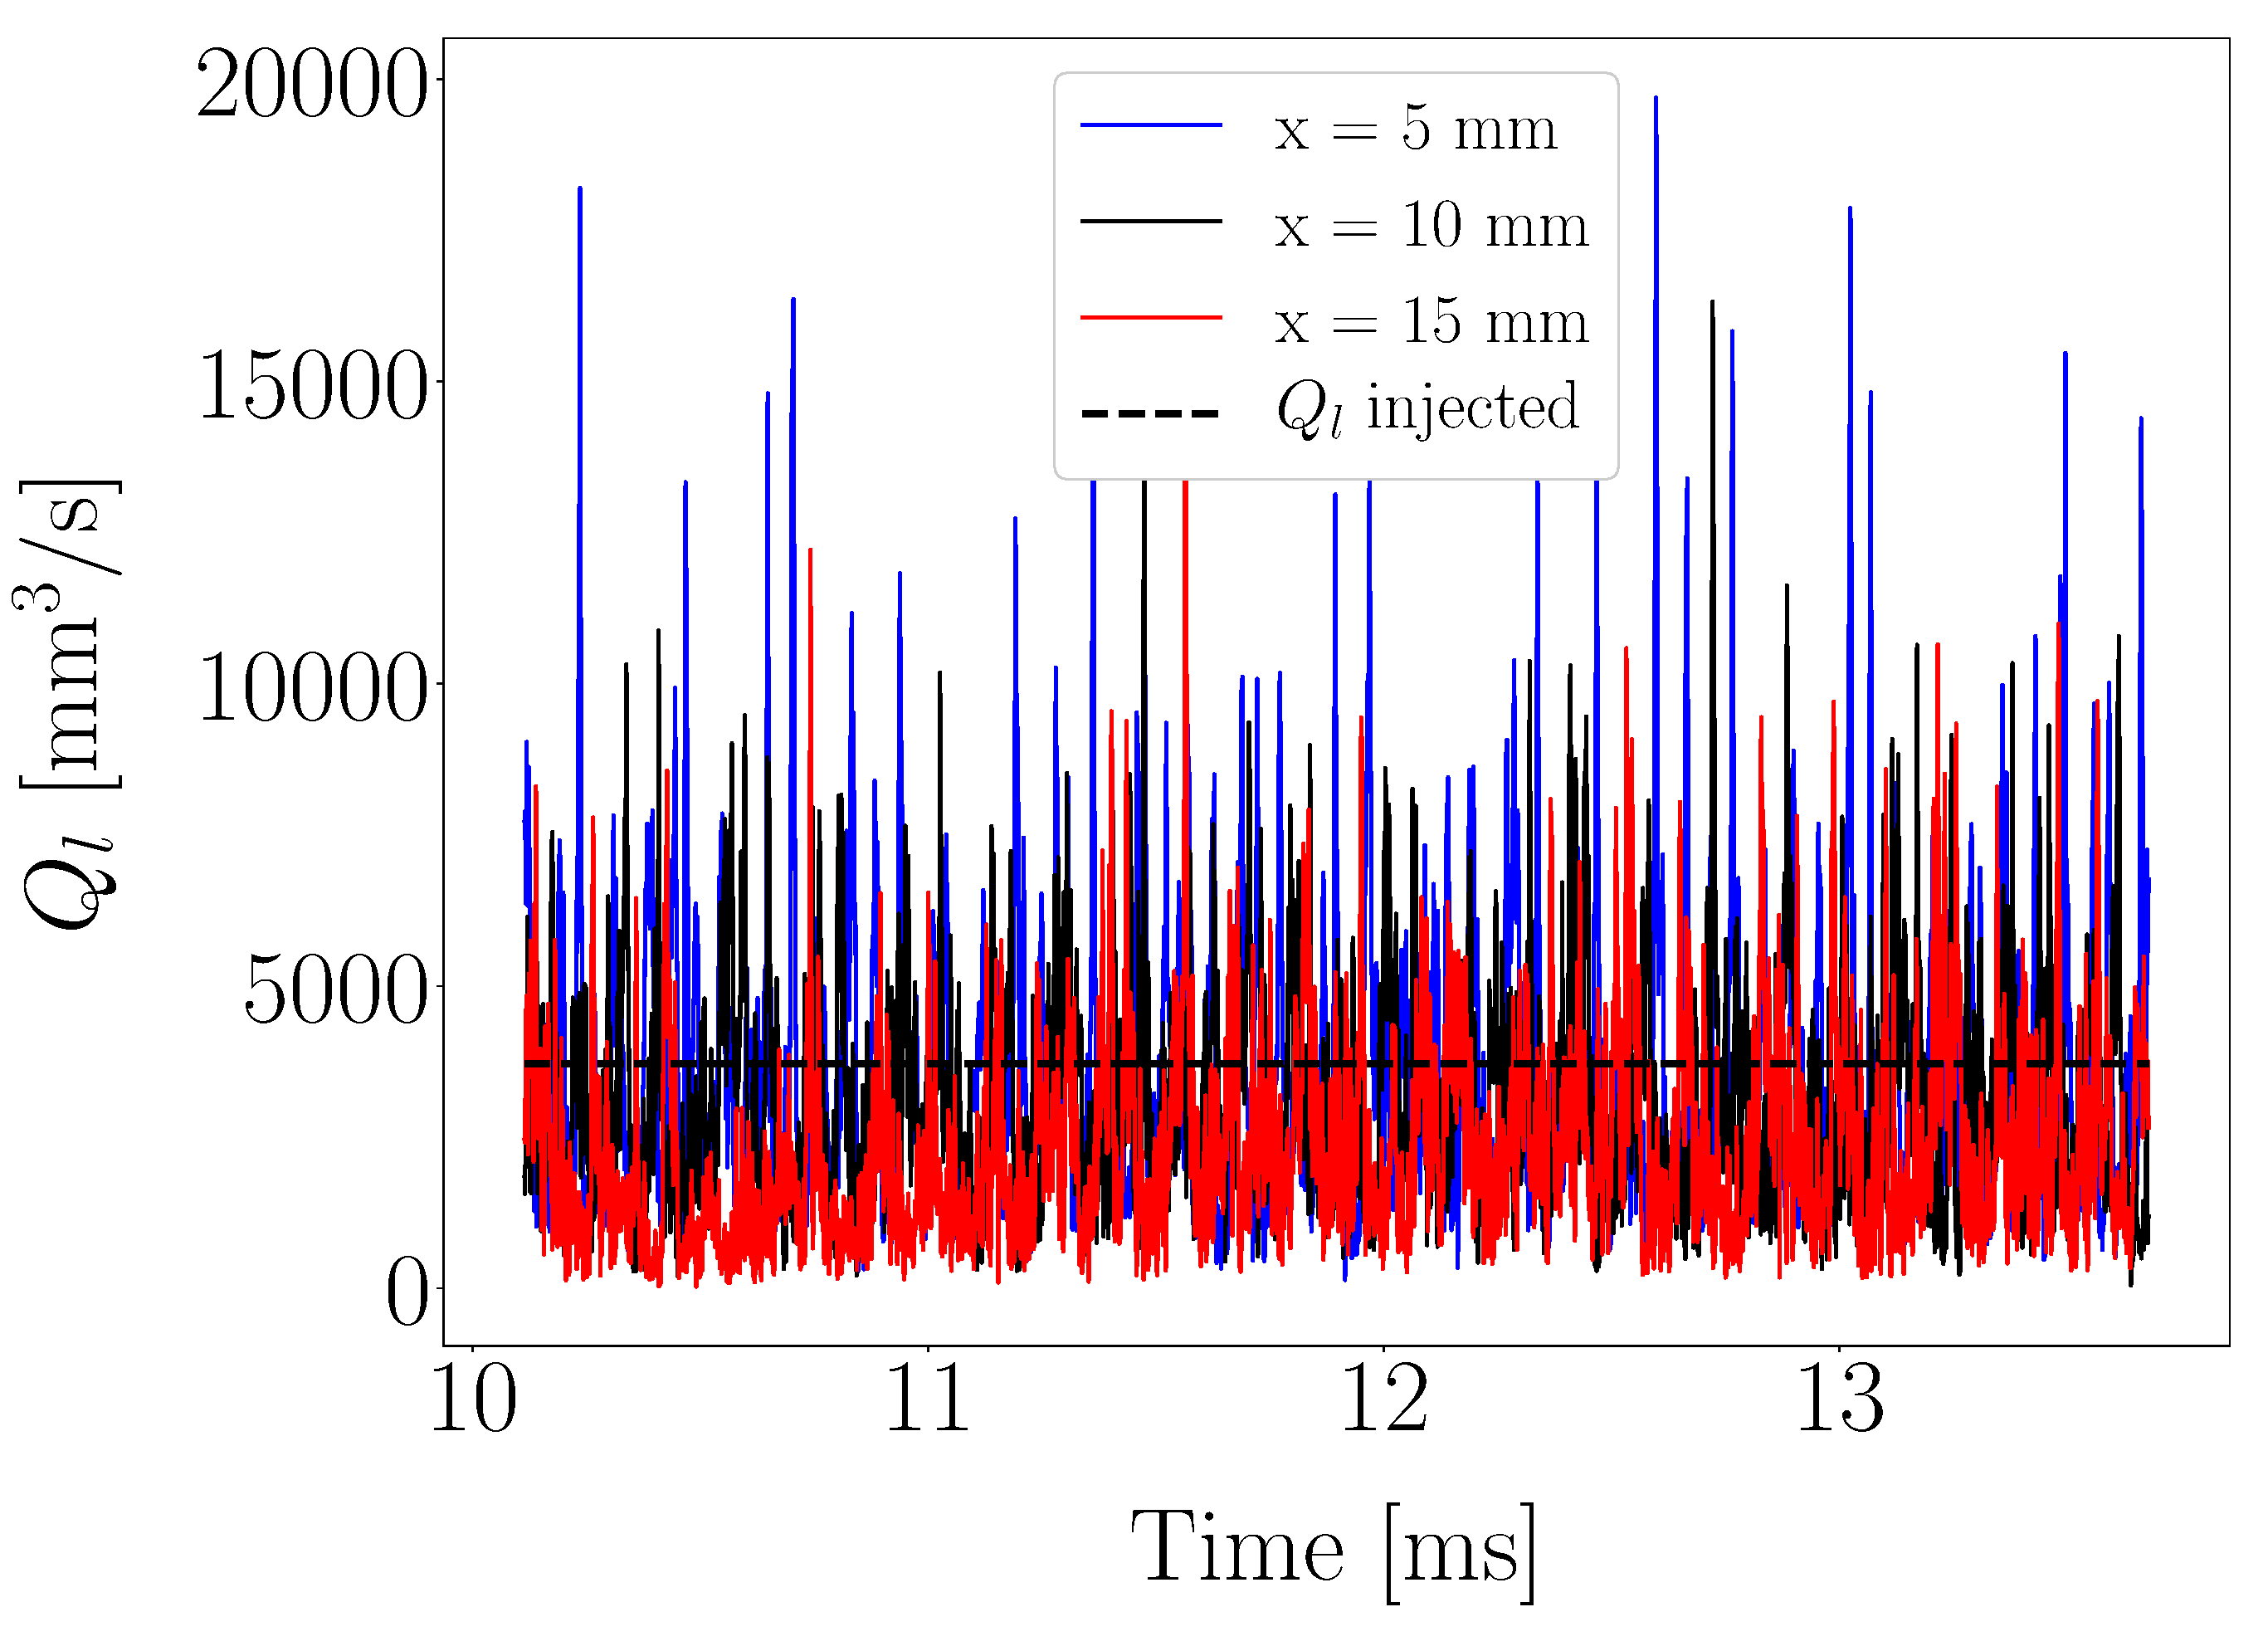
\includegraphics[scale=0.6]{./part2_developments/figures_ch5_resolved_JICF/flow_rates_ibs/uG100_dx20_QL_isox_time_evol.eps}
%\caption{Liquid flow rate evolution with time in the}
%\label{fig:graphite_cp}
%\end{figure}

\begin{figure}[ht]
\centering
\begin{subfigure}[b]{0.45\textwidth}
	\centering
   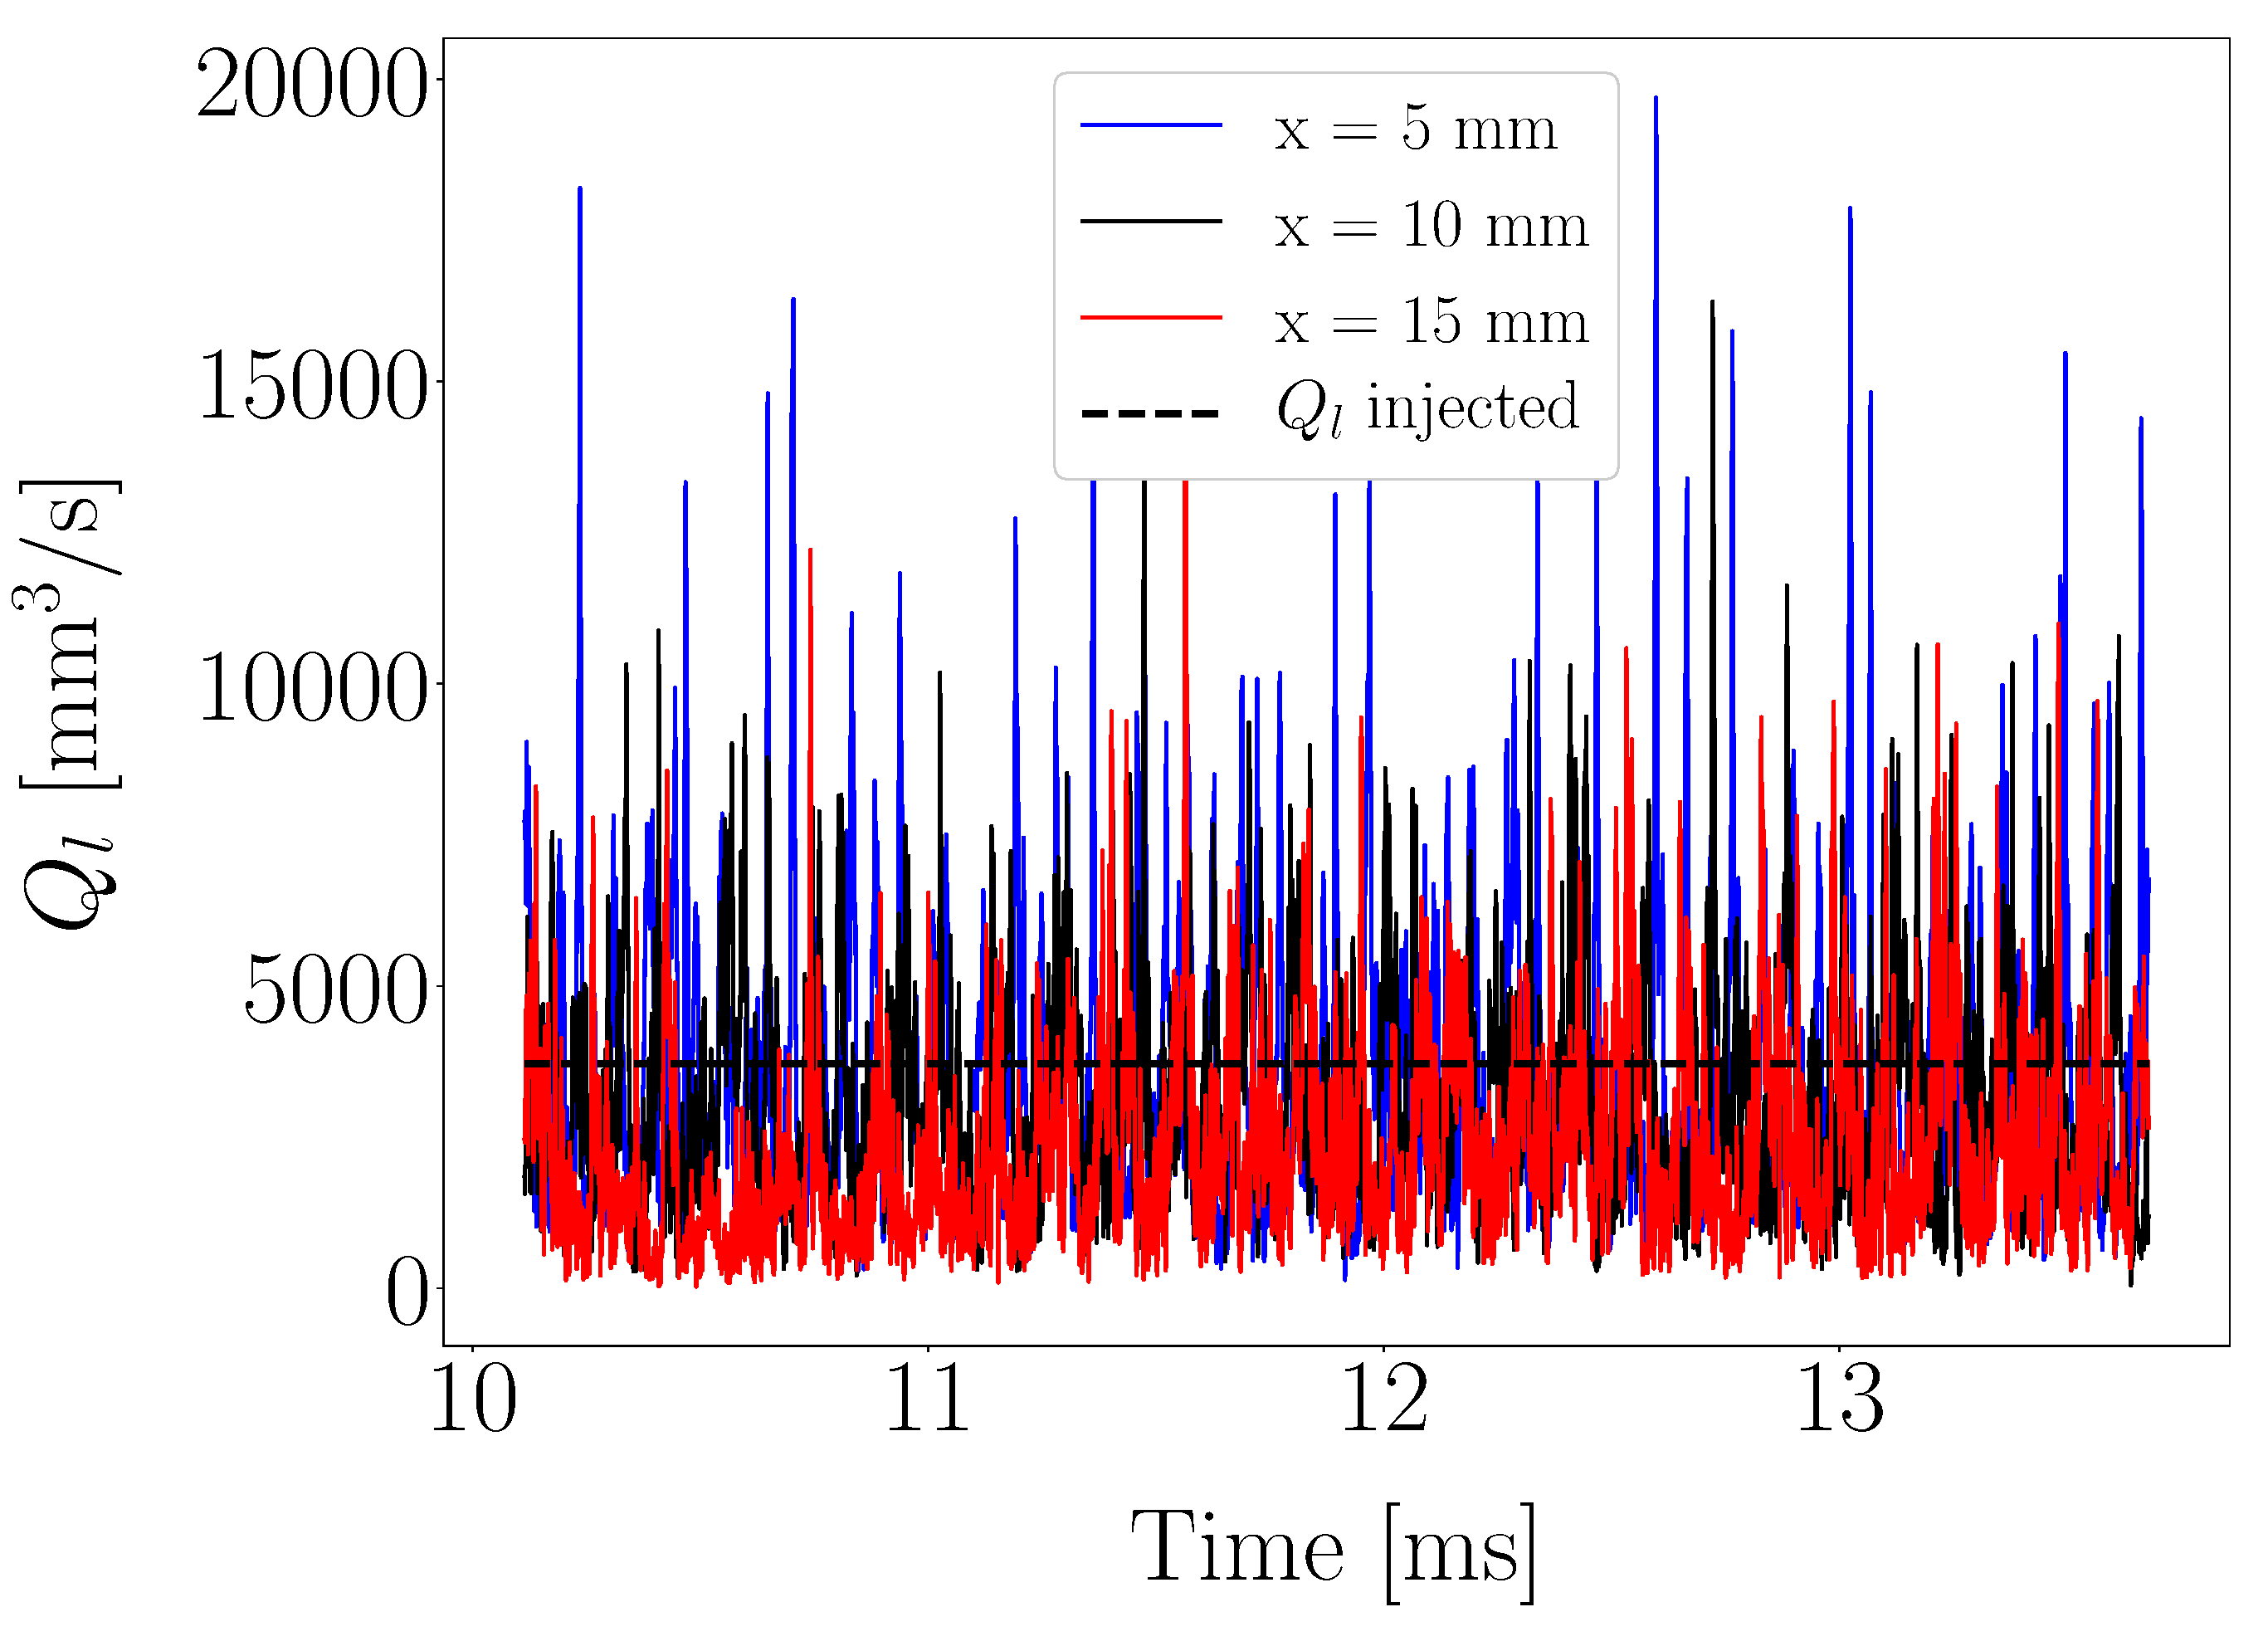
\includegraphics[scale=0.15]{./part2_developments/figures_ch5_resolved_JICF/flow_rates_ibs/uG100_dx20_QL_isox_time_evol.eps}
   %\caption{}
   %\label{} 
\end{subfigure}
\begin{subfigure}[b]{0.45\textwidth}
	\centering
   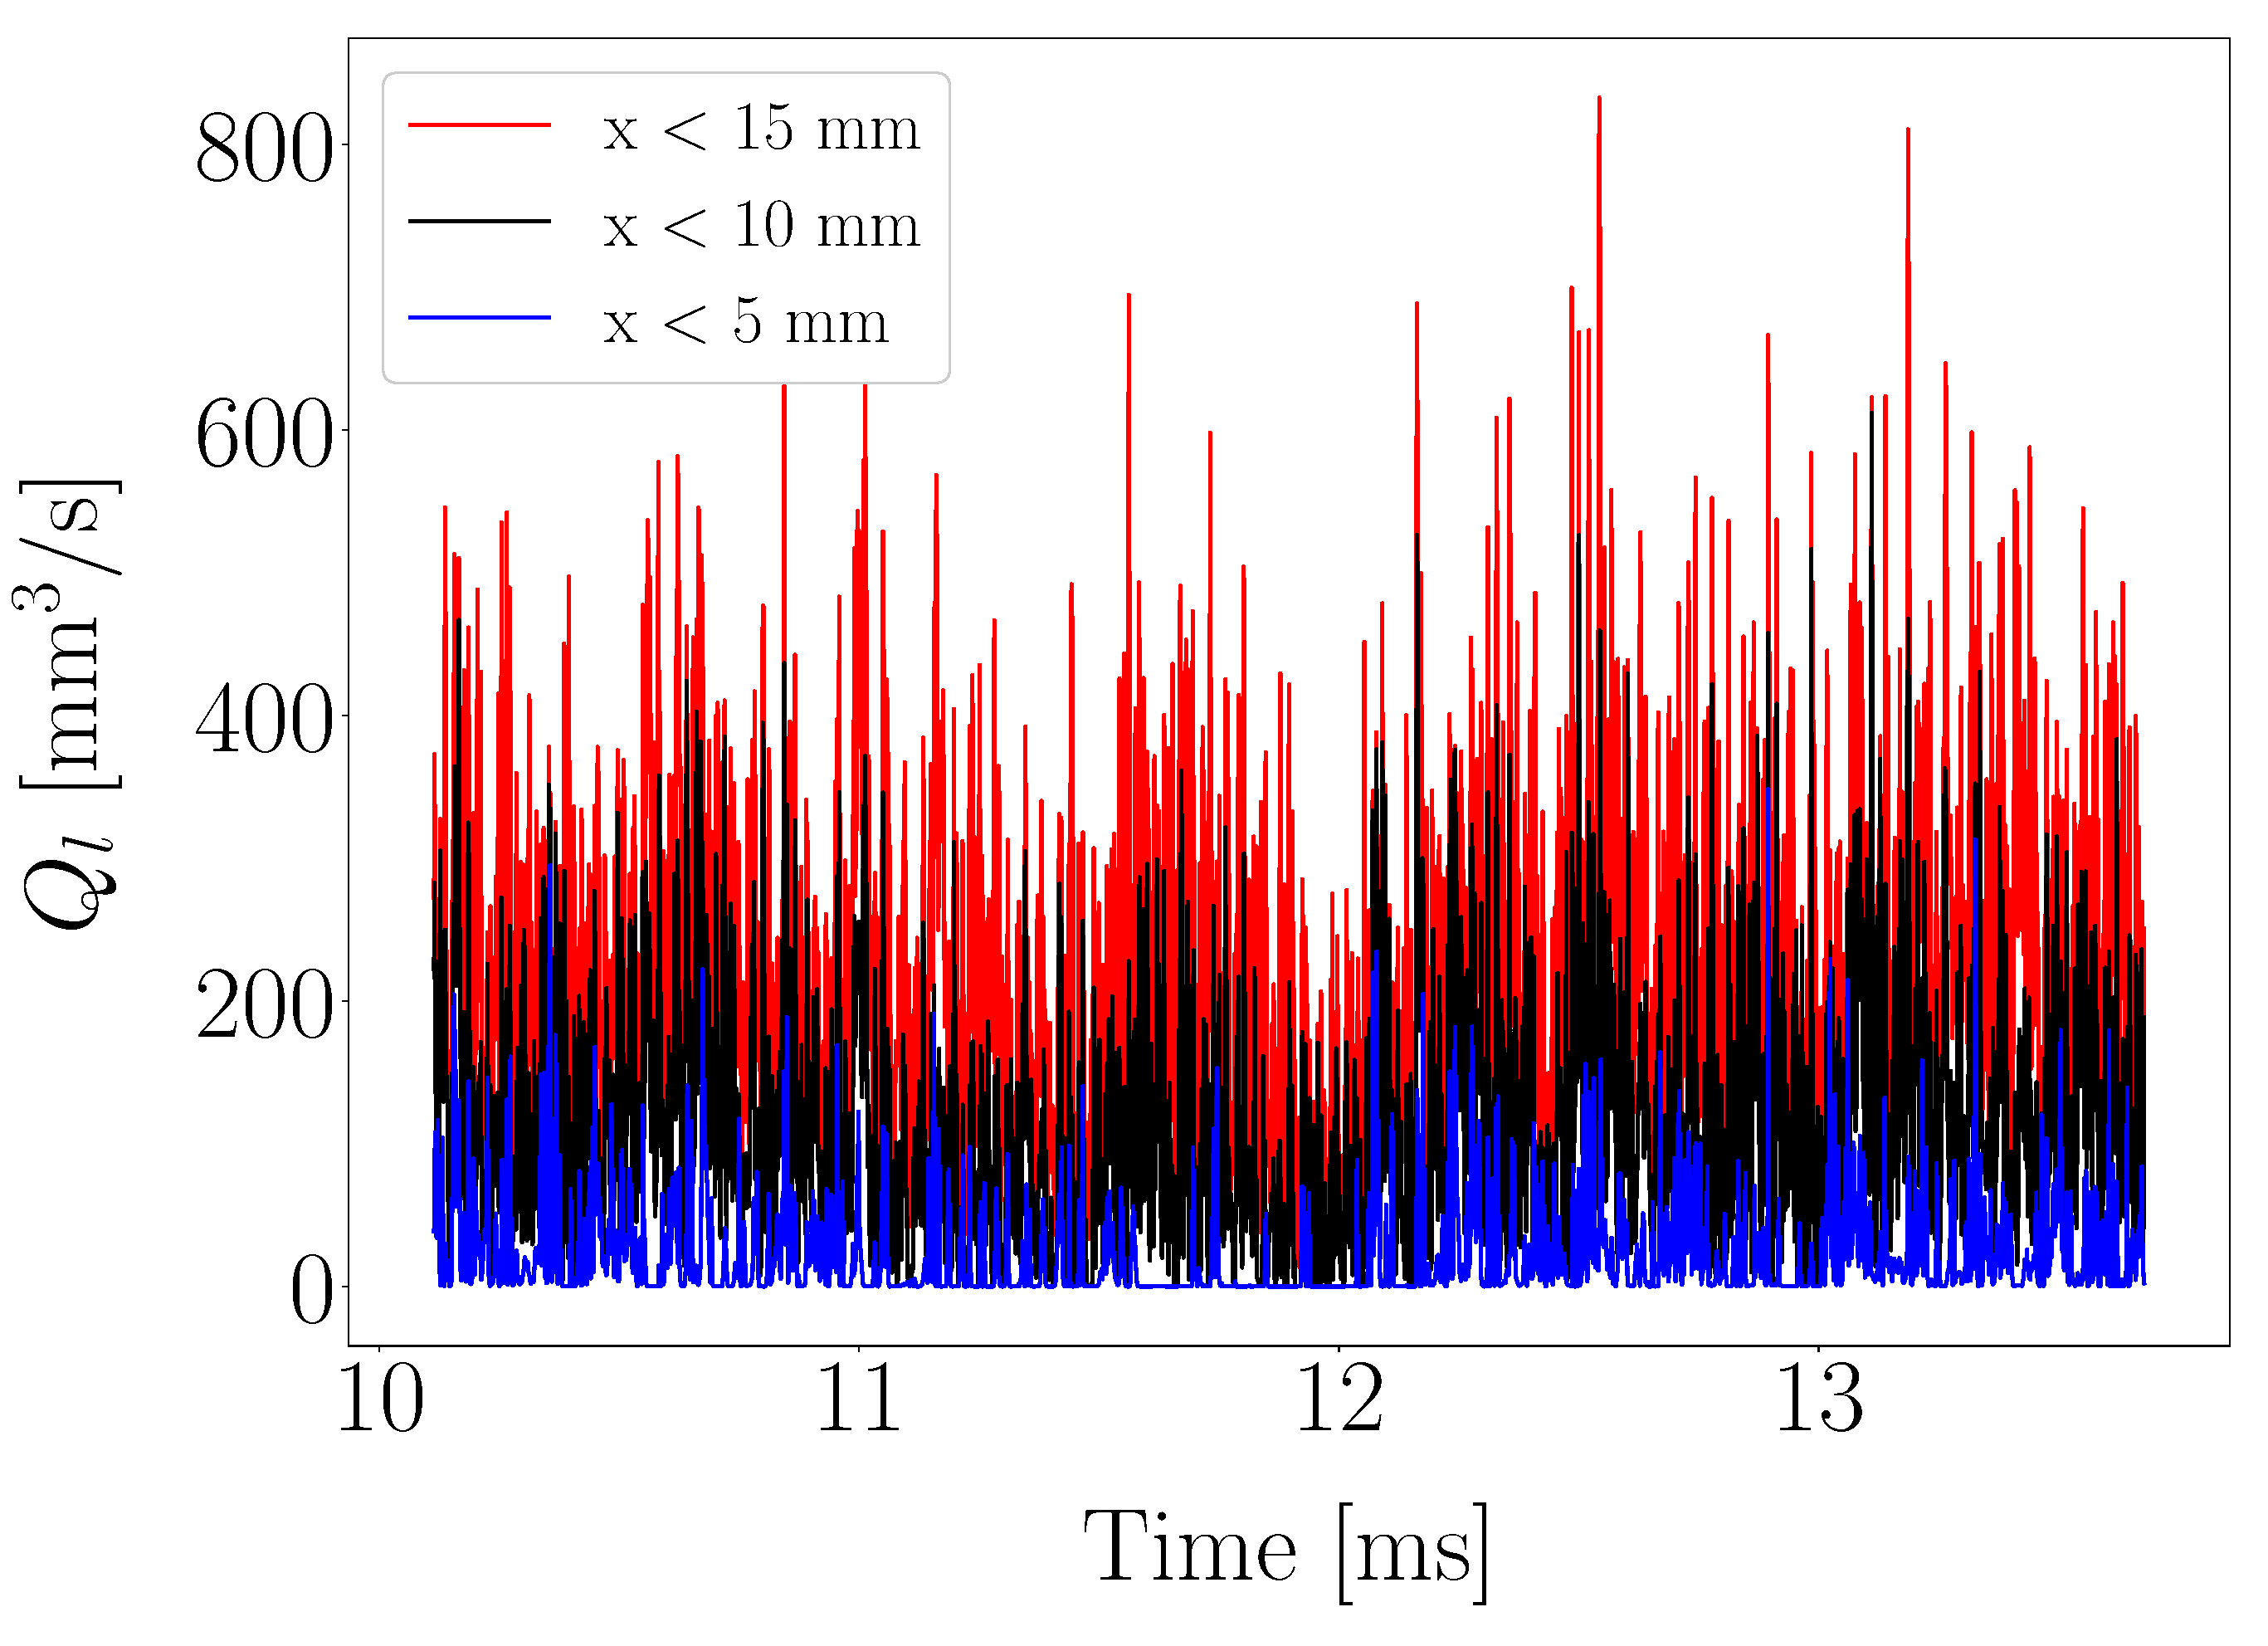
\includegraphics[scale=0.15]{./part2_developments/figures_ch5_resolved_JICF/flow_rates_ibs/uG100_dx20_QL_filming_time_evol.eps}
   %\caption{}
   %\label{}
\end{subfigure}
\caption{Time evolution of instantaneous liquid flow rates for case UG100\_DX20. \textbf{Left}: planes normal to crossflow. \textbf{Right}: filming planes.}
\label{fig:IB_liquid_flow_rate_inst_evolution_UG100_DX20}
\end{figure}

\begin{figure}[ht]
\centering
\begin{subfigure}[b]{0.45\textwidth}
	\centering
   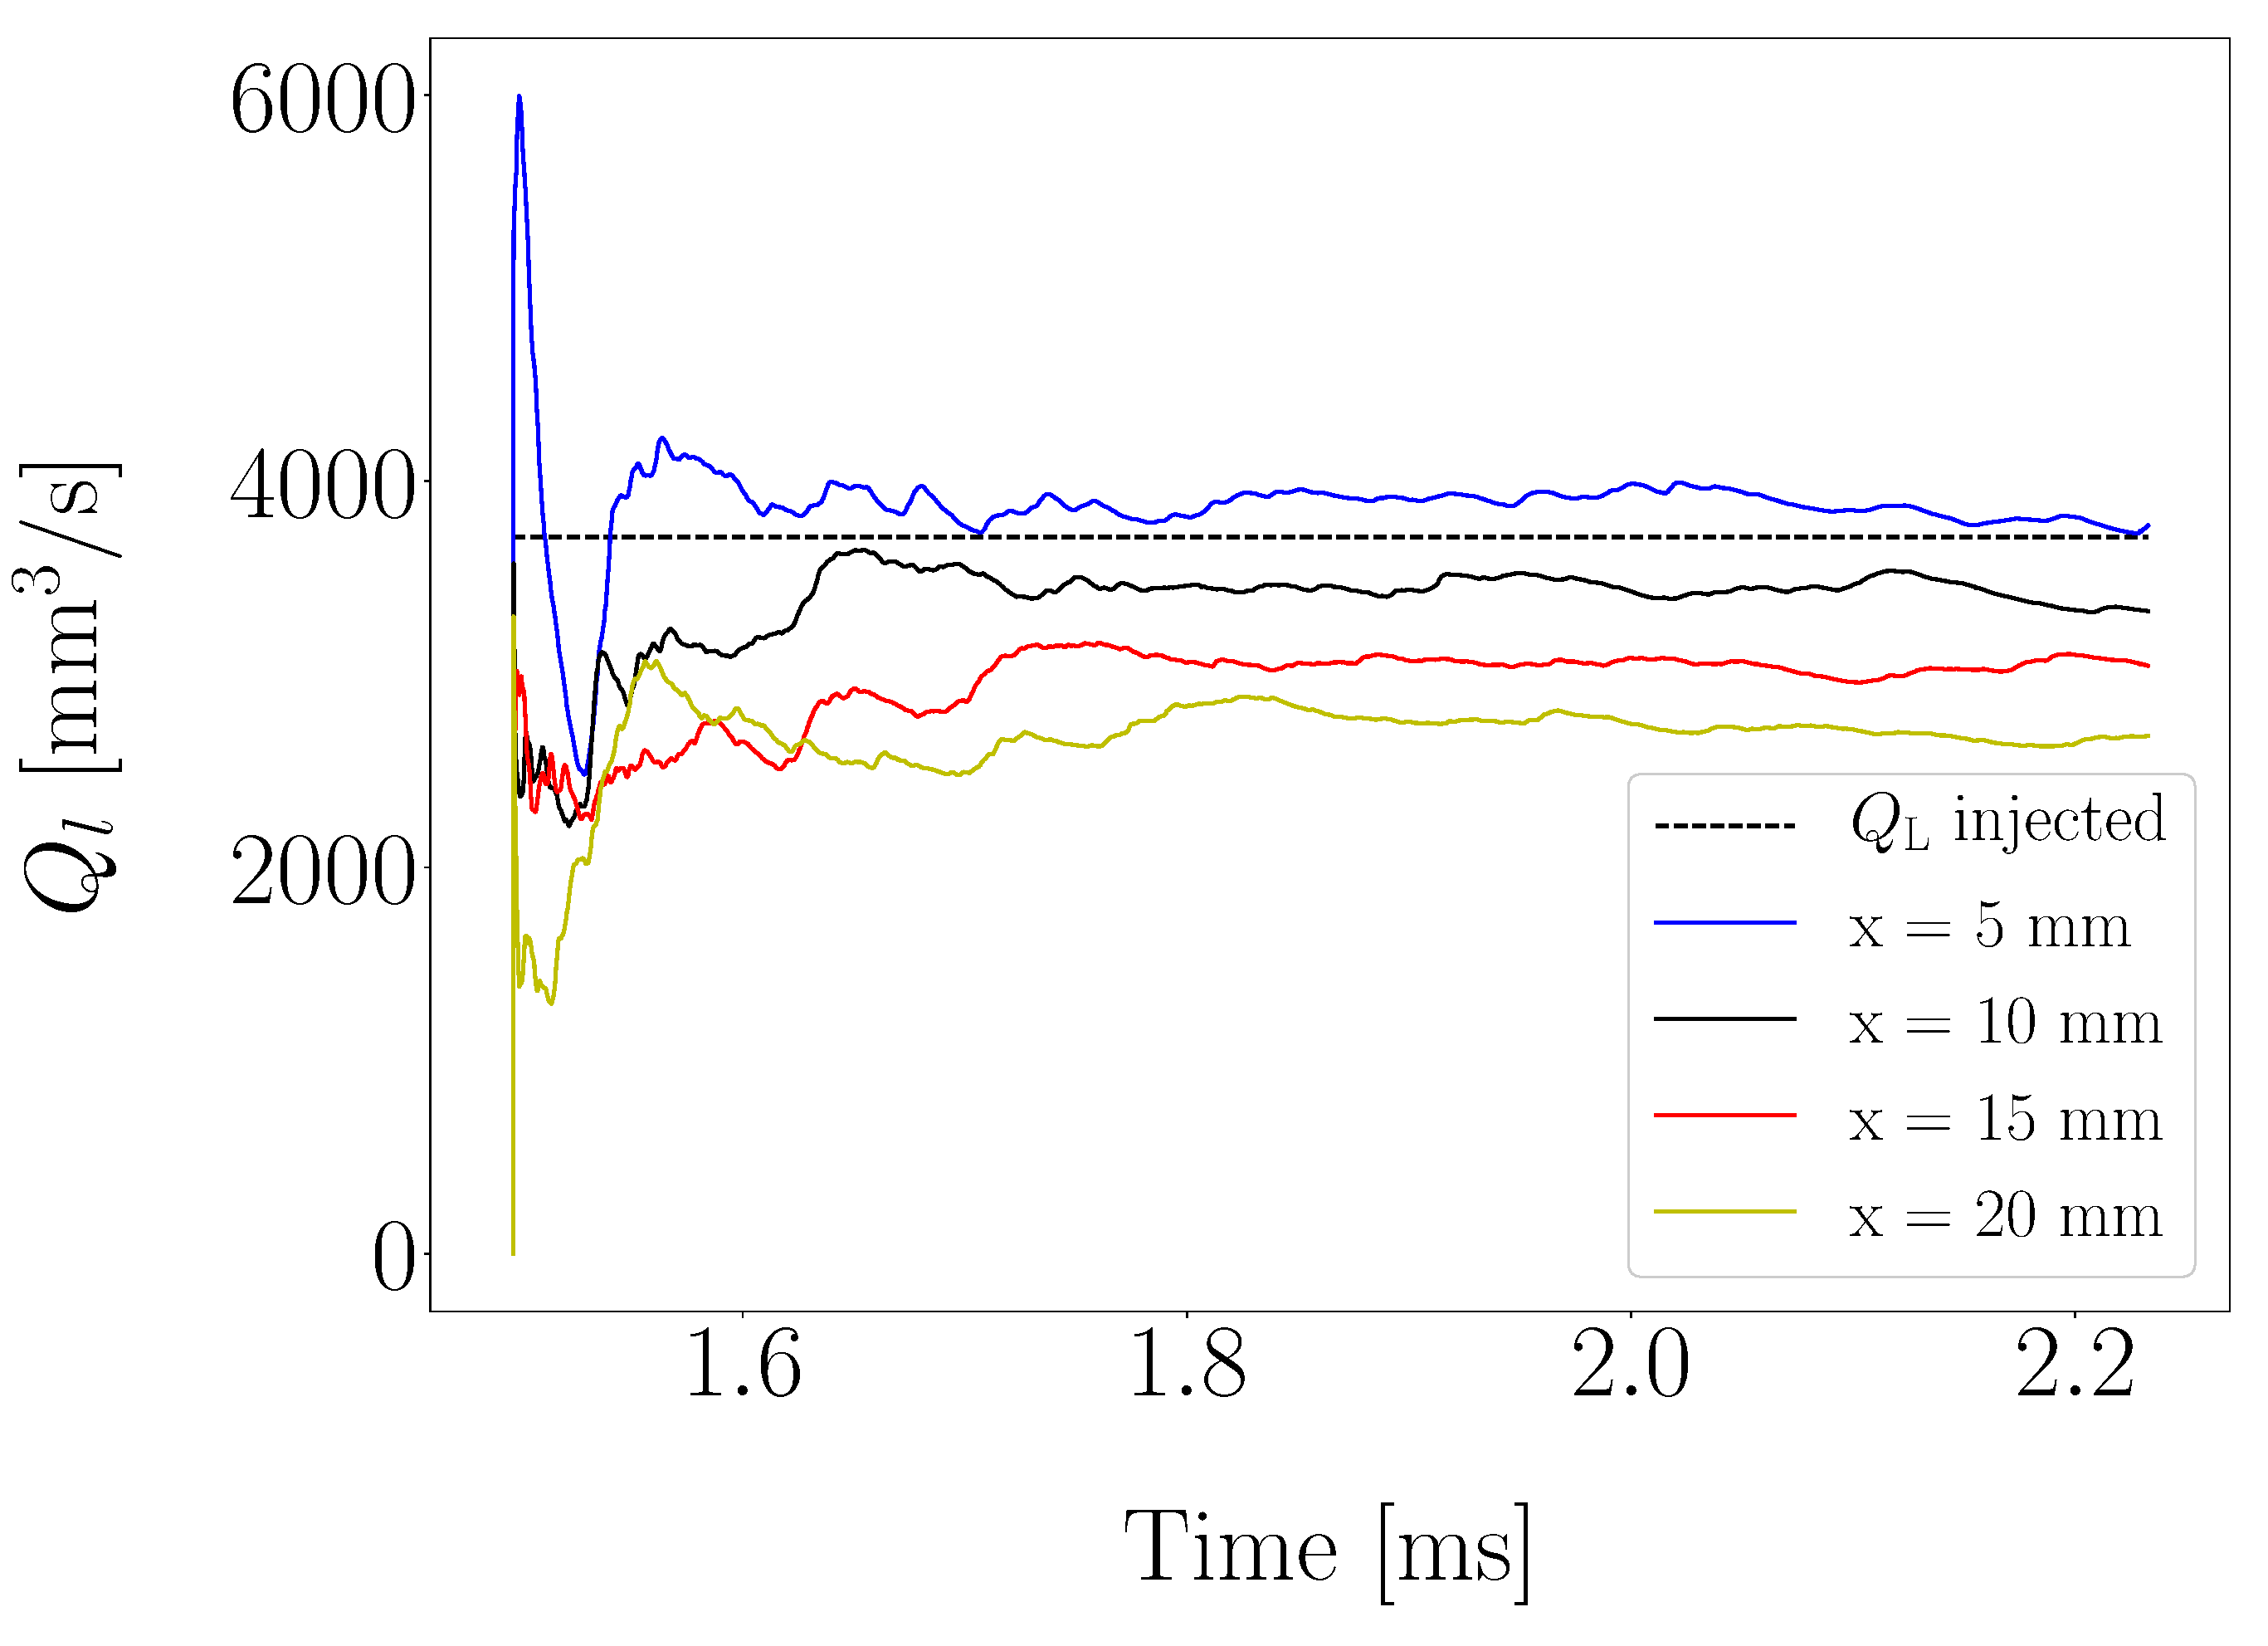
\includegraphics[scale=0.17]{./part2_developments/figures_ch5_resolved_JICF/flow_rates_ibs/uG100_dx20_QL_isox_mean_time_convergence.eps}
   \caption{Mean $Q_l$ in crossflow planes}
   %\label{} 
\end{subfigure}
\hfill
\begin{subfigure}[b]{0.45\textwidth}
	\centering
   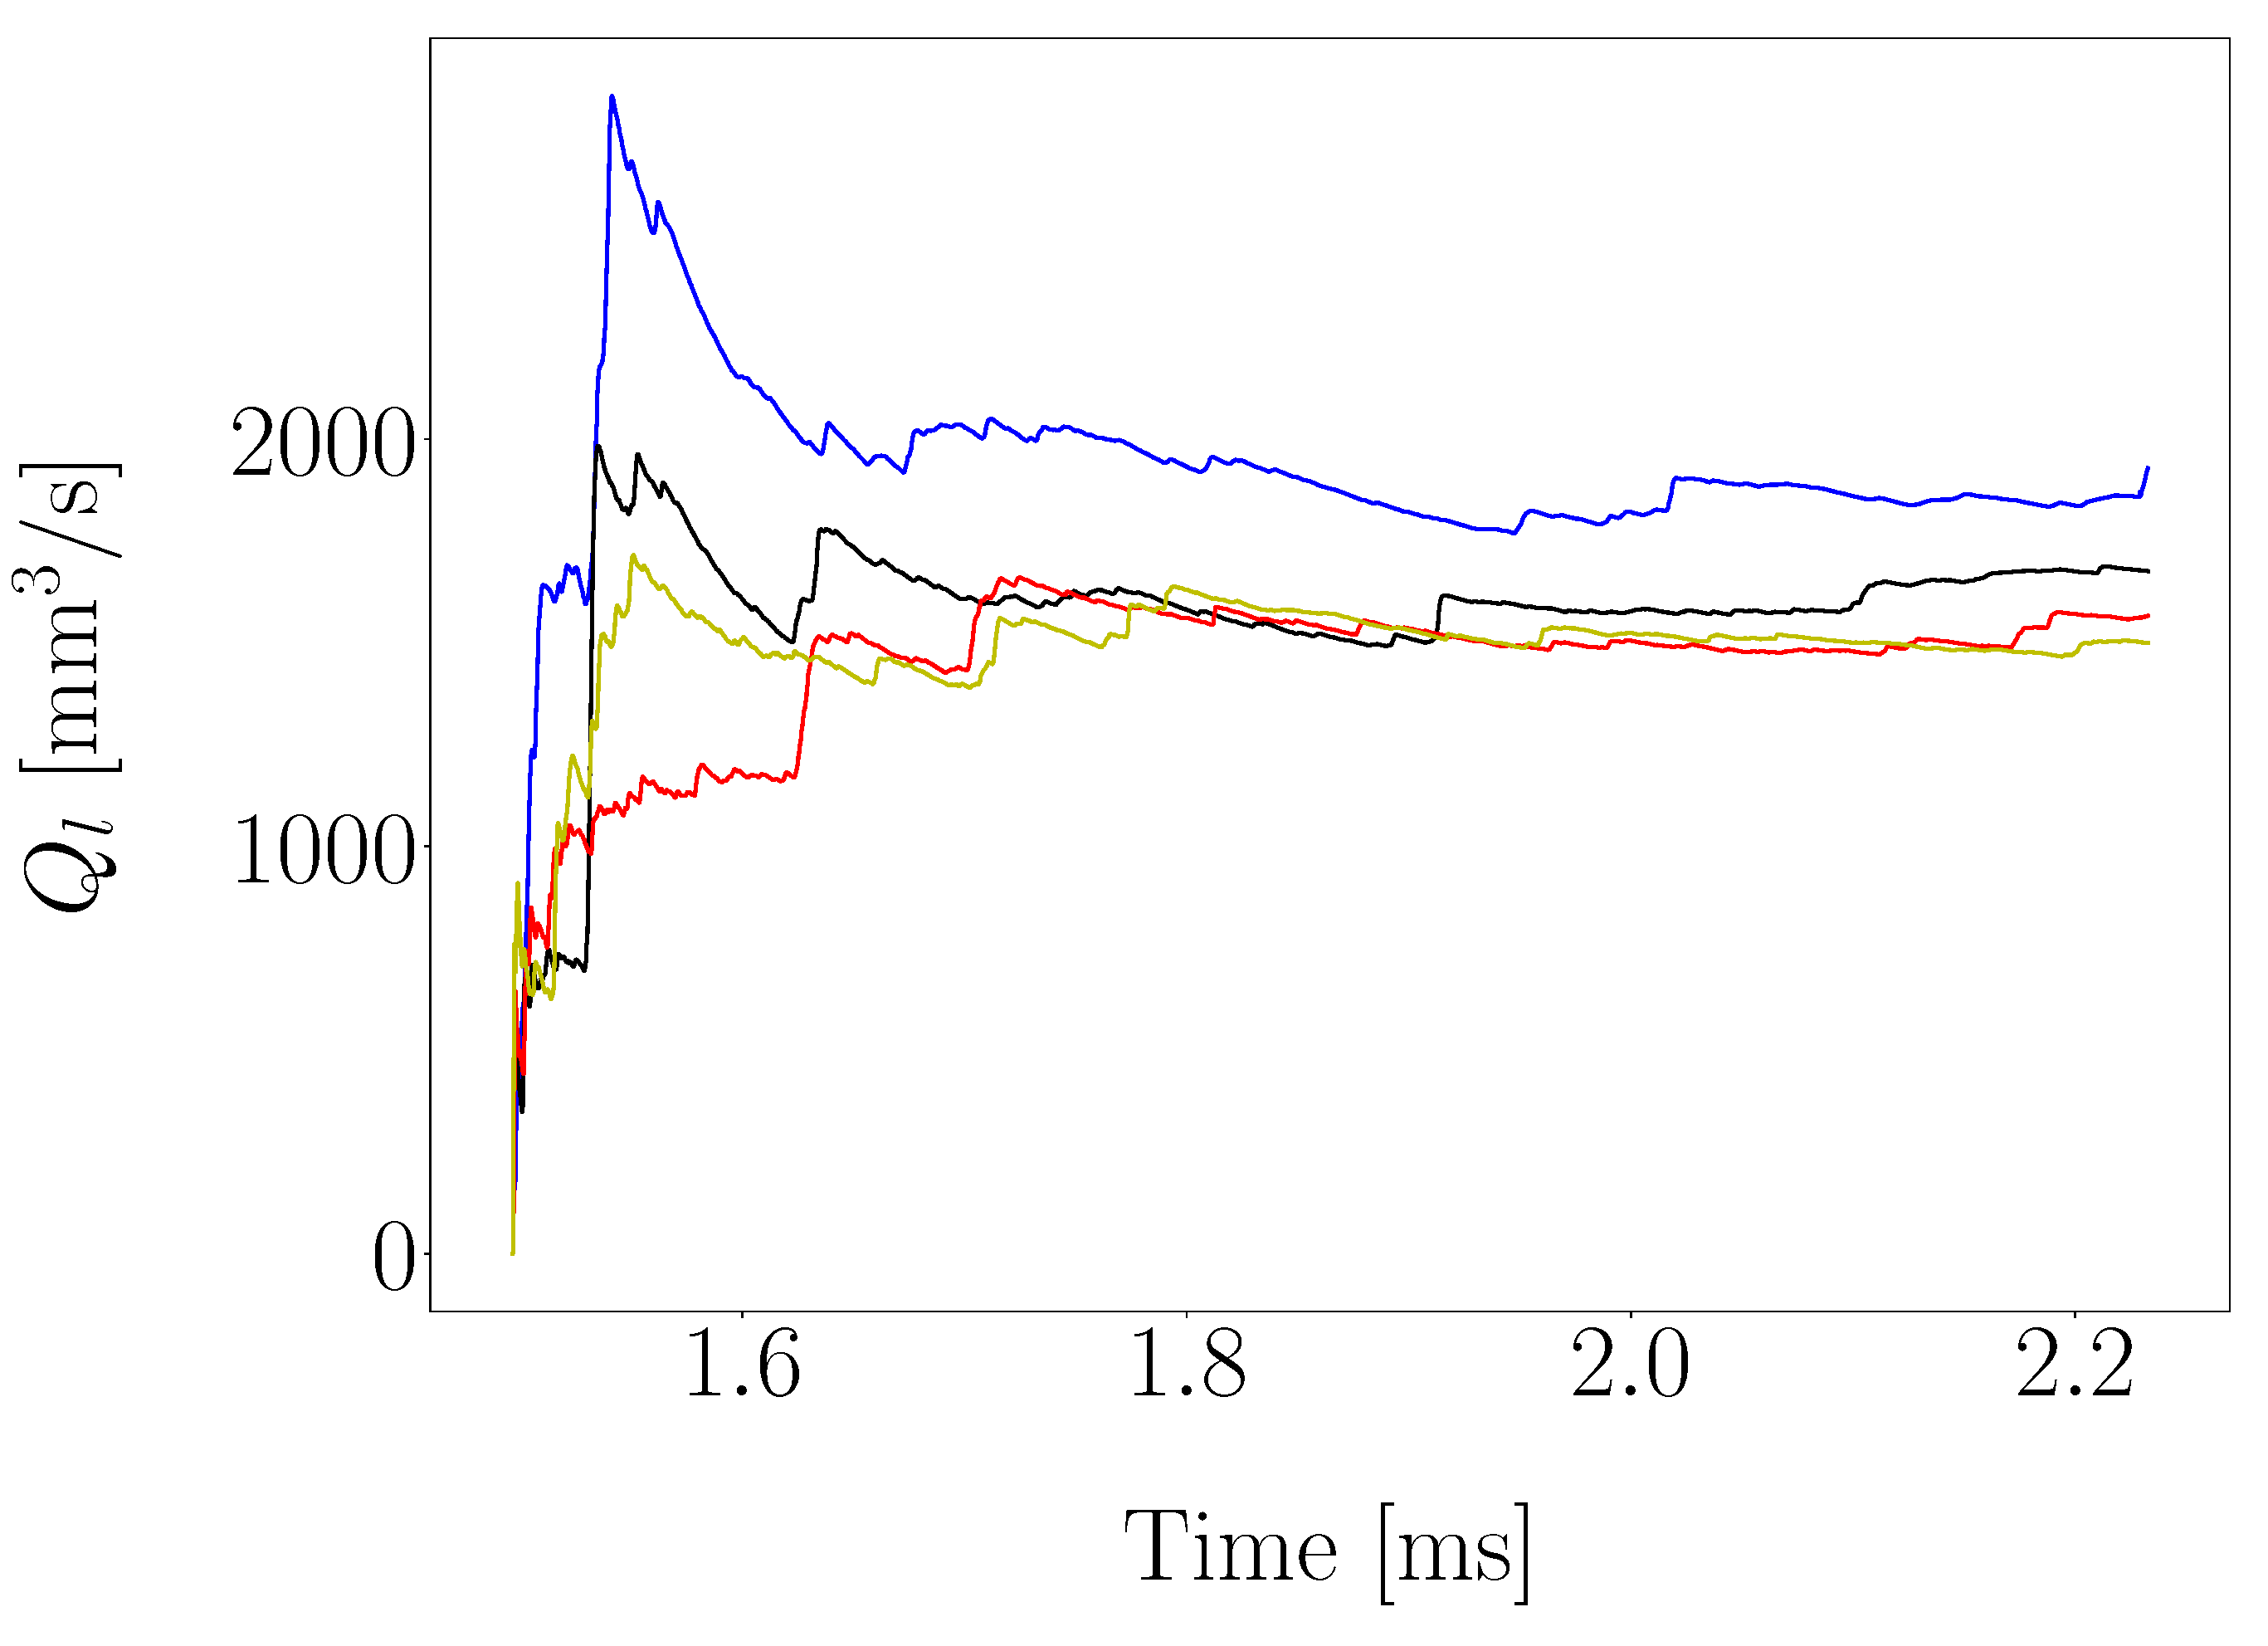
\includegraphics[scale=0.17]{./part2_developments/figures_ch5_resolved_JICF/flow_rates_ibs/uG100_dx20_QL_isox_RMS_time_convergence.eps}
   \caption{RMS $Q_l$ in crossflow planes}
   %\label{}
\end{subfigure}
\vskip\baselineskip
\begin{subfigure}[b]{0.45\textwidth}
	\centering
   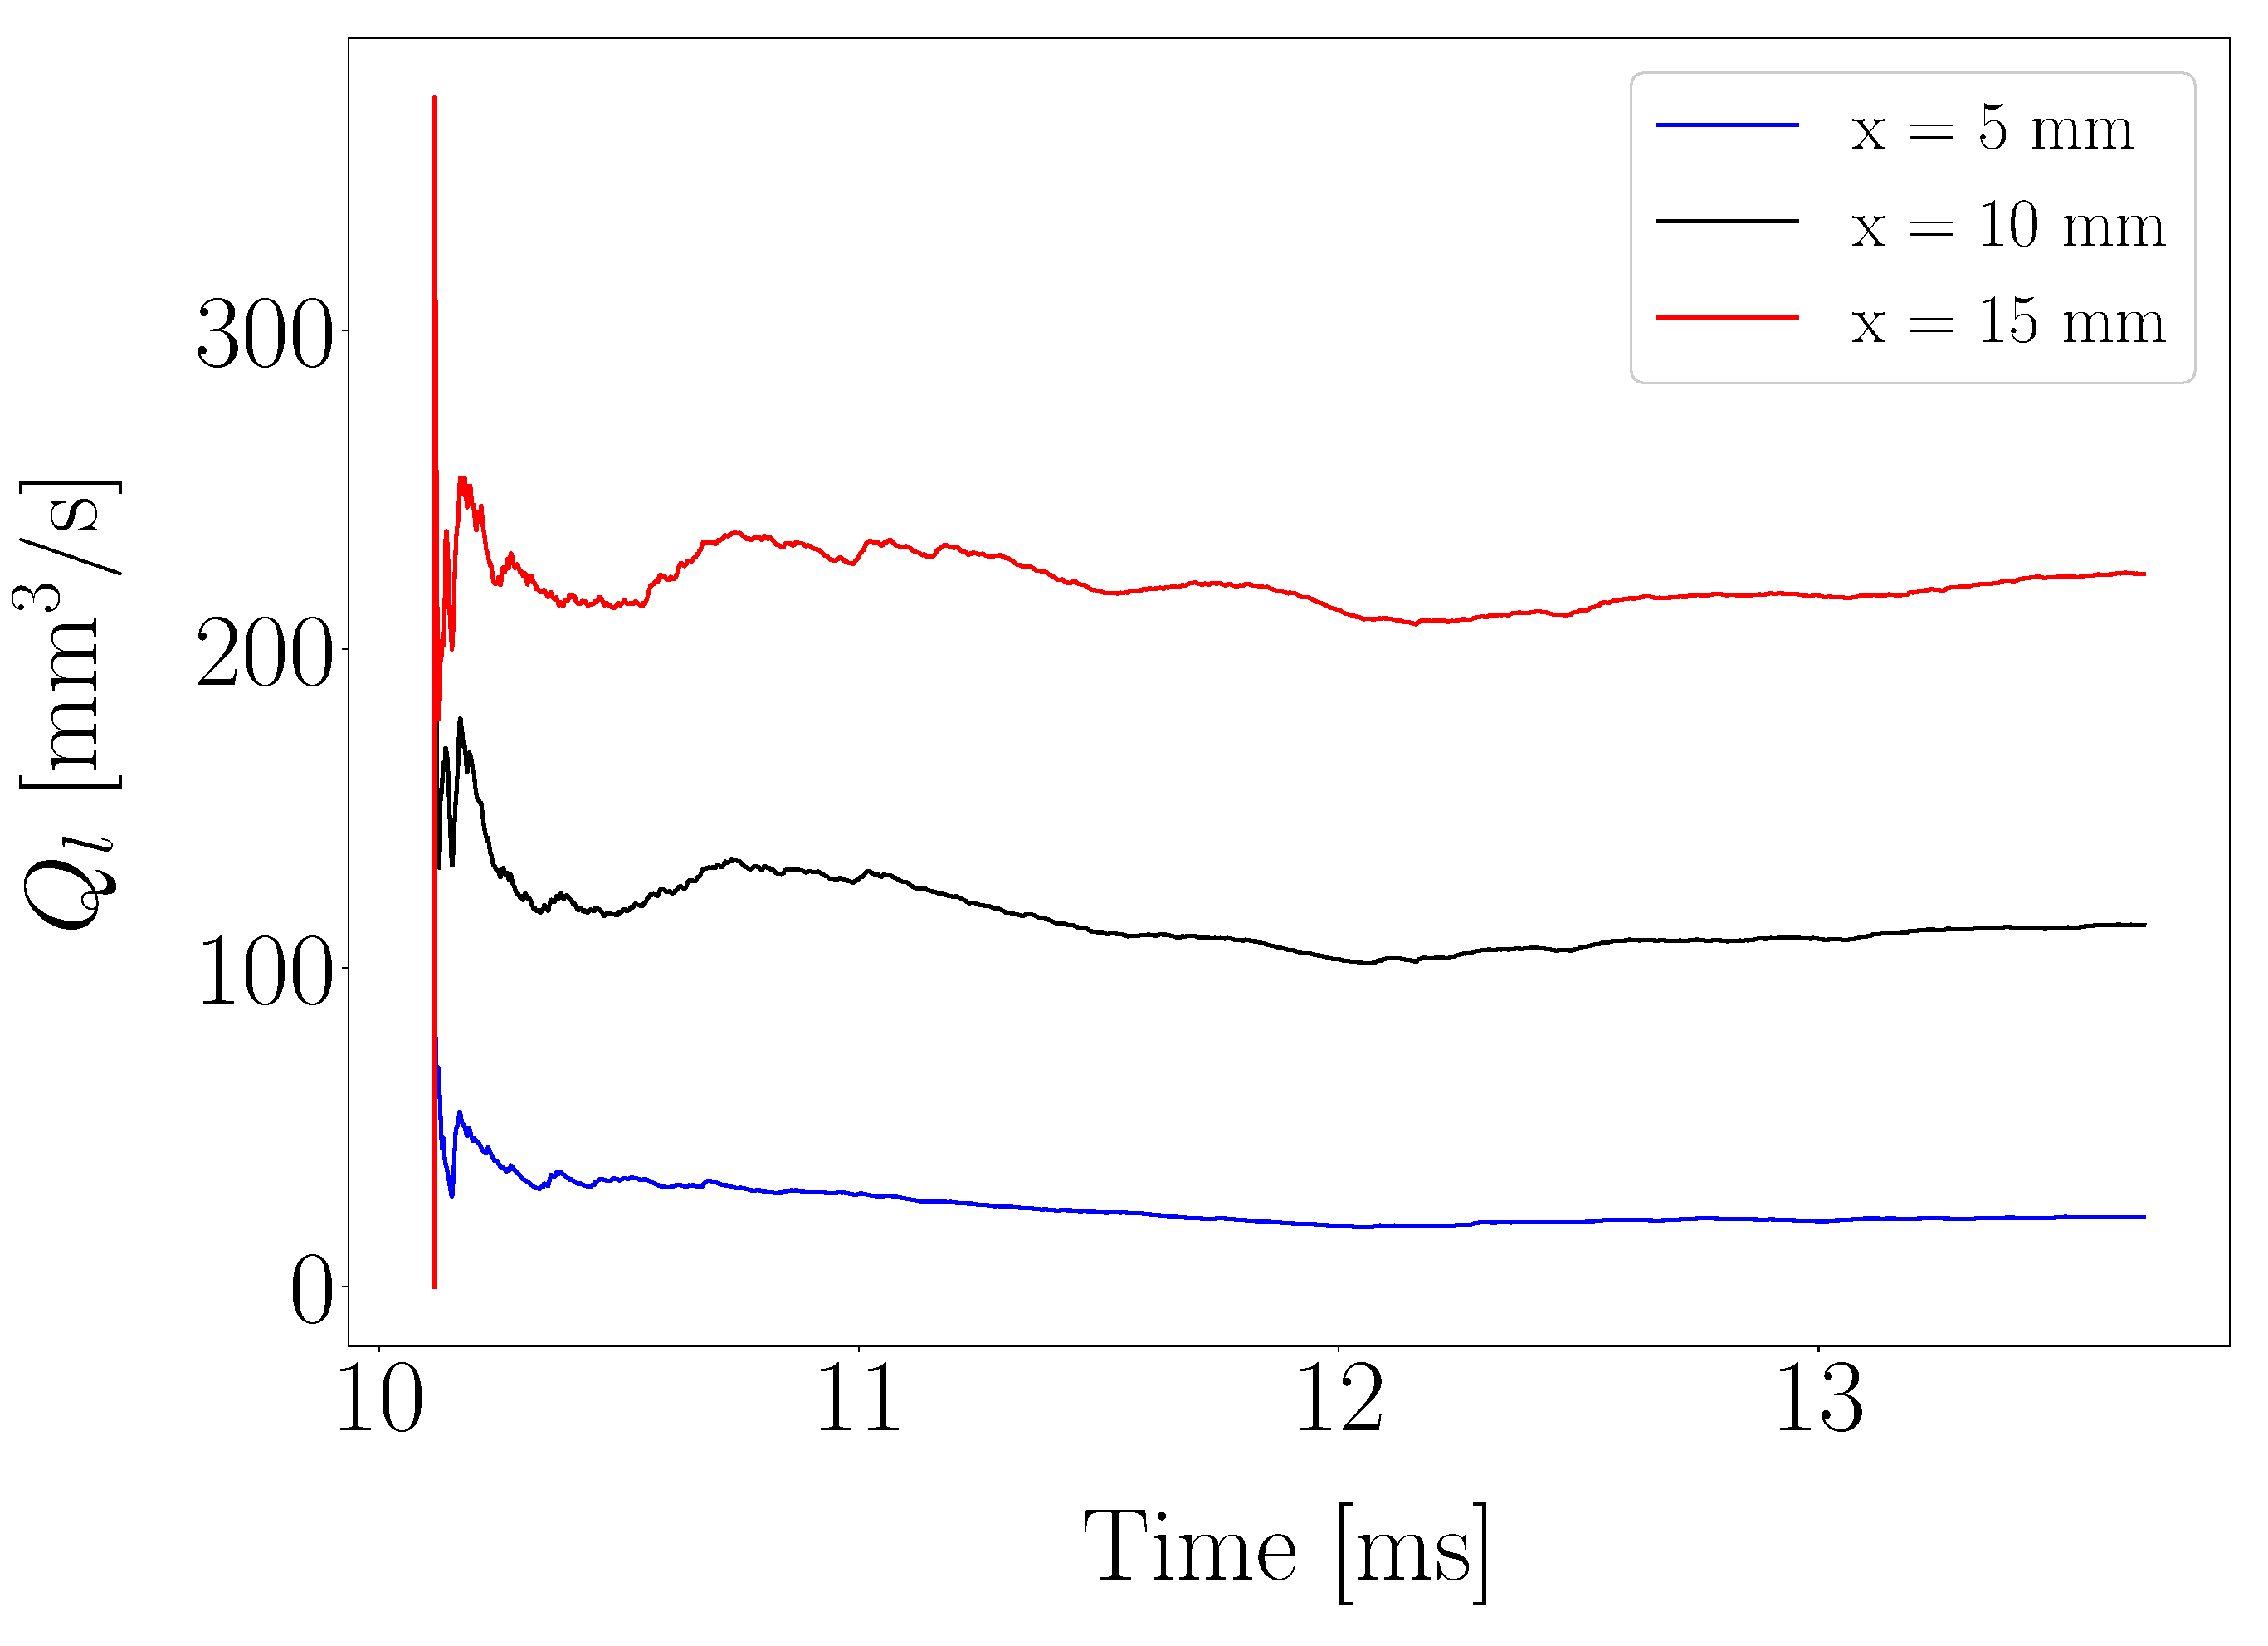
\includegraphics[scale=0.17]{./part2_developments/figures_ch5_resolved_JICF/flow_rates_ibs/uG100_dx20_QL_filming_mean_time_convergence.eps}
   \caption{Mean $Q_l$ in filming planes}
   %\label{} 
\end{subfigure}
\hfill
\begin{subfigure}[b]{0.45\textwidth}
	\centering
   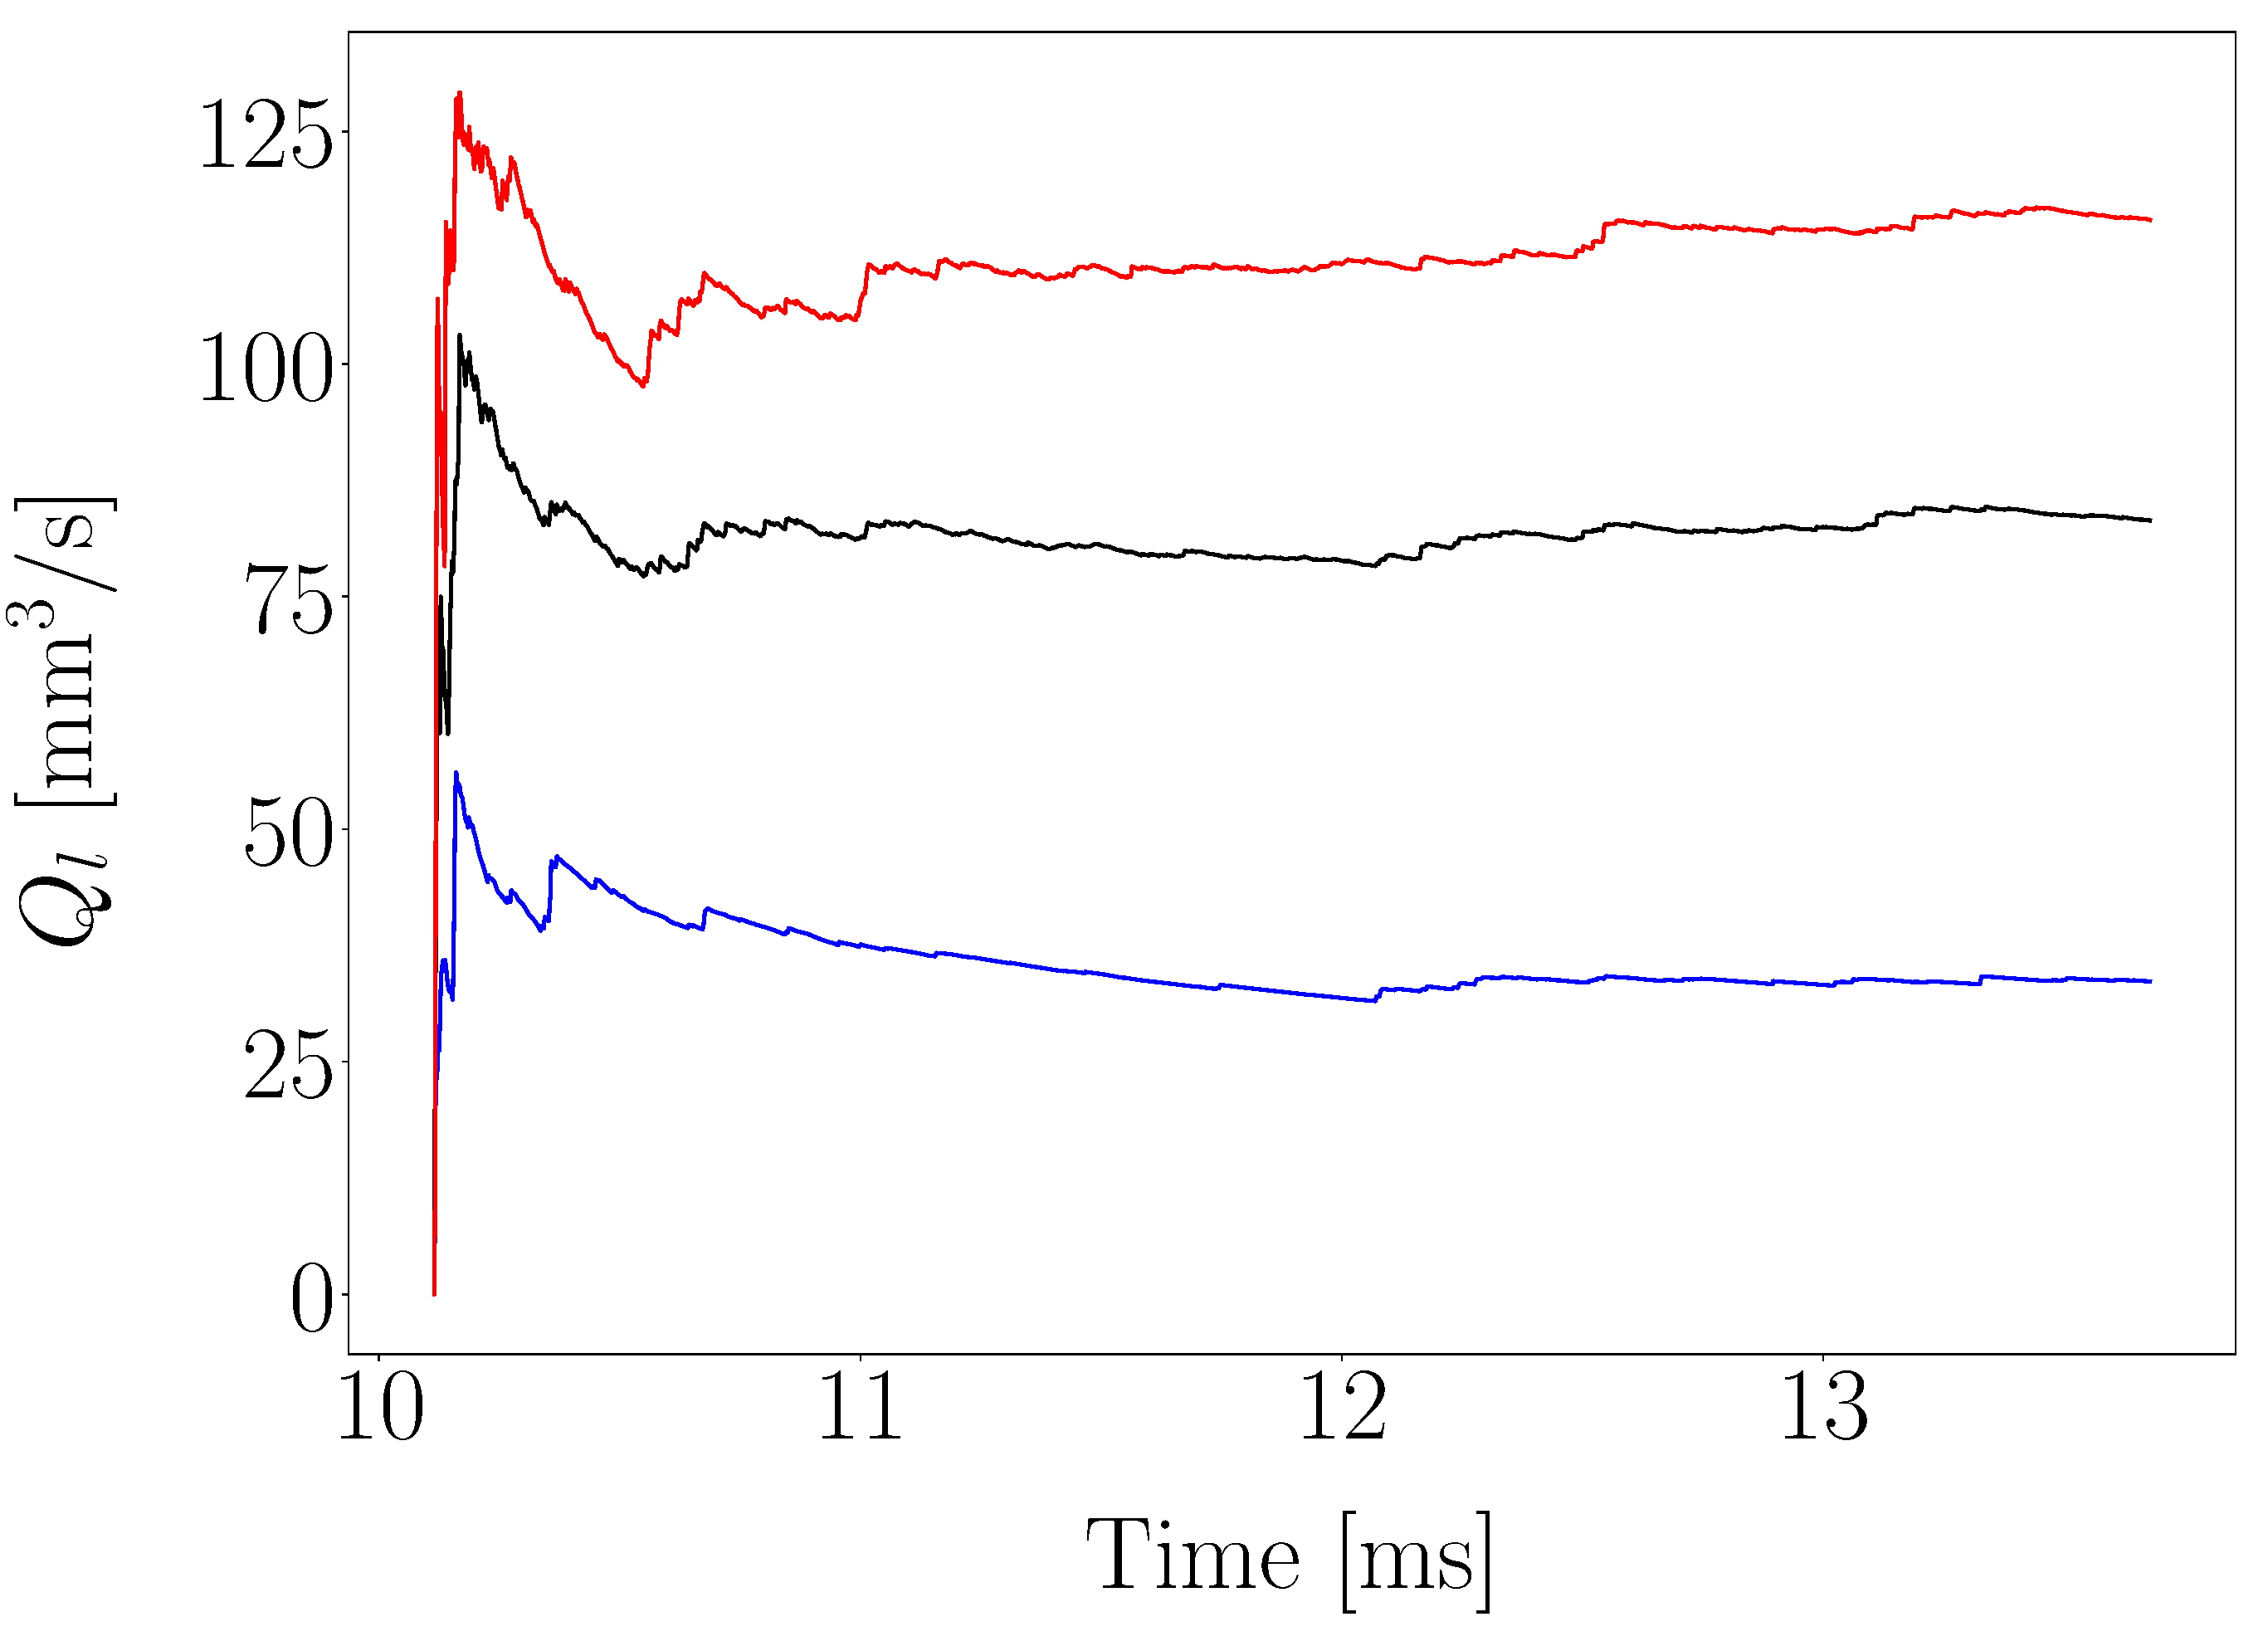
\includegraphics[scale=0.17]{./part2_developments/figures_ch5_resolved_JICF/flow_rates_ibs/uG100_dx20_QL_filming_RMS_time_convergence.eps}
   \caption{RMS $Q_l$ in filming planes}
   %\label{}
\end{subfigure}
\caption{Time evolution of mean and RMS liquid flow rates for case UG100\_DX20.}
\label{fig:IB_liquid_flow_rate_mean_RMS_evolution_UG100_DX20}
\end{figure}


\begin{figure}[ht]
\centering
\begin{subfigure}[b]{0.45\textwidth}
	\centering
   \includegraphics[scale=0.10]{./part2_developments/figures_ch5_resolved_JICF/flow_rates_ibs/uG100_dx20_QL_isox_bar_plot.eps}
   \caption{Case UG100\_DX20: crossflow planes}
   %\label{} 
\end{subfigure}
\hfill
\begin{subfigure}[b]{0.45\textwidth}
	\centering
   \includegraphics[scale=0.10]{./part2_developments/figures_ch5_resolved_JICF/flow_rates_ibs/uG100_dx20_QL_filming_bar_plot.eps}
   \caption{Case UG100\_DX20: filming planes}
   %\label{}
\end{subfigure}
\vskip\baselineskip
\begin{subfigure}[b]{0.45\textwidth}
	\centering
   \includegraphics[scale=0.10]{./part2_developments/figures_ch5_resolved_JICF/flow_rates_ibs/uG100_dx10_QL_isox_bar_plot.eps}
   \caption{Case UG100\_DX10: crossflow planes}
   %\label{} 
\end{subfigure}
\hfill
\begin{subfigure}[b]{0.45\textwidth}
	\centering
   \includegraphics[scale=0.10]{./part2_developments/figures_ch5_resolved_JICF/flow_rates_ibs/uG100_dx10_QL_filming_bar_plot.eps}
   \caption{Case UG100\_DX10: filming planes}
   %\label{}
\end{subfigure}

\vskip\baselineskip

\begin{subfigure}[b]{0.45\textwidth}
	\centering
   \includegraphics[scale=0.10]{./part2_developments/figures_ch5_resolved_JICF/flow_rates_ibs/uG75_dx20_QL_isox_bar_plot.eps}
   \caption{Case UG75\_DX20: crossflow planes}
   %\label{} 
\end{subfigure}
\hfill
\begin{subfigure}[b]{0.45\textwidth}
	\centering
   \includegraphics[scale=0.10]{./part2_developments/figures_ch5_resolved_JICF/flow_rates_ibs/uG75_dx20_QL_filming_bar_plot.eps}
   \caption{Case UG75\_DX20: filming planes}
   %\label{}
\end{subfigure}
\vskip\baselineskip
\begin{subfigure}[b]{0.45\textwidth}
	\centering
   \includegraphics[scale=0.10]{./part2_developments/figures_ch5_resolved_JICF/flow_rates_ibs/uG75_dx10_QL_isox_bar_plot.eps}
   \caption{Case UG75\_DX10: crossflow planes}
   %\label{} 
\end{subfigure}
\hfill
\begin{subfigure}[b]{0.45\textwidth}
	\centering
   \includegraphics[scale=0.10]{./part2_developments/figures_ch5_resolved_JICF/flow_rates_ibs/uG75_dx10_QL_filming_bar_plot.eps}
   \caption{Case UG75\_DX10: filming planes}
   %\label{}
\end{subfigure}
\caption[Mean flow rates (bars) and RMS (lines) obtained with interior boundaries for each simulation performed]{Mean flow rates (bars) and RMS (lines) obtained with interior boundaries for each simulation performed. }
\label{fig:JICF_ibs_flow_rates_bars_plots}
\end{figure}









\subsubsection*{Spatial distribution of flow rates in crossflow planes}






\subsection{Mass conservation in ACLS}

%\subsubsection{Sampling procedure for droplets}


\subsection{Spray characterization}


\subsubsection{Droplets size distributions}

Show histograms with lognormal fit (from Lefebvre equation and from optimal fit).

\subsubsection{Definition of characteristic times}

Several characteristic times can be defined in a jet in crossflow:

\begin{itemize}

	\item Characteristic time of ligaments passage at given planes, $t_\mathrm{pas}$
	
	\item Characteristic time related to the frequency of the instabilities causing column breakup, $t_\mathrm{ins}$
	
	\item Physical definition according to ...

\end{itemize}



\subsection{Gaseous field and dense core characterization}
\label{subsec:ch5_dense_core_in_ACLS_simus}

\subsection{Frequential analysis}

A spectral analysis is performed to obtain the characteristic breakup frequencies. There are several ways to obtain the desired frequencies:

\begin{itemize}

	\item Use Proper Orthogonal Decomposition (POD) technique (2018 Prakash, Mukundan). This is out of the scope of this work.
	
	\item Get evolution of breakup point with time: $x_b \left( t \right)$, $z_b \left( t \right)$, then get the frequency spectrum  (2010 Wang, 2018 Prakash). Not sure we can do this with our available data, so not envisageable now.
	
	\item Locate probes along liquid column, get liquid presence rate with time. This is the one !!

\end{itemize}

\subsection{Computational performances}
\label{subsec:ch5_computational_performances}

%\subsection{Feeding the models (??)}
%Find a more attractive name

\section{Learning injectors}

\subsection{Spatial discretization of sprays}

%\subsection{Operating point at high We}
%
%\subsection{Operating point at low We}


\section{Conclusions}

